\documentclass[conference]{IEEEtran}

\usepackage{amsmath,amssymb,amsfonts}
\usepackage{algorithmic}
\usepackage{graphicx}
\usepackage{textcomp}
\usepackage{xcolor}
\usepackage{booktabs}
\usepackage{multirow}
\usepackage{array}
\usepackage{cite}
\usepackage{url}
\usepackage{bm}

\title{ANN-Based Adaptive Source Coding with Systematic LDPC Channel Coding for Lossless Wired Communication}

\author{\IEEEauthorblockN{Ganesh M}
\IEEEauthorblockA{\textit{School of Computer Science and Engineering}\\
\textit{VIT-AP University}\\
Amaravati, Andhra Pradesh, India \\
ganesh.23bce8887@vitapstudent.ac.in}
\and
\IEEEauthorblockN{Muhammad Sajid Y}
\IEEEauthorblockA{\textit{School of Computer Science and Engineering}\\
\textit{VIT-AP University}\\
Amaravati, Andhra Pradesh, India \\
sajid.23bce7802@vitapstudent.ac.in}
\and
\IEEEauthorblockN{Komali Priya P}
\IEEEauthorblockA{\textit{School of Computer Science and Engineering}\\
\textit{VIT-AP University}\\
Amaravati, Andhra Pradesh, India \\
priya.23bce9973@vitapstudent.ac.in}
\and
\IEEEauthorblockN{Dr. M.Mahesh}
\IEEEauthorblockA{\textit{School of Electronics Engineering}\\
\textit{VIT-AP University}\\
Amaravati, Andhra Pradesh, India \\
mahesh.m@vitap.ac.in}
}

\begin{document}

\maketitle

% =========================================================================
% ABSTRACT
% =========================================================================
\begin{abstract}
High-throughput wired interconnects, SerDes telemetry buses, and industrial automation networks encounter heterogeneous traffic profiles ranging from structured JSON payloads to compiled machine code and incompressible encrypted data. Traditional communication architectures rely on static source codecs and legacy linear block codes such as Hamming(7,4), which underperform when source statistics vary and experience decoding breakdowns under impulsive electromagnetic interference (EMI). In this paper, we propose an integrated framework combining \textbf{Artificial Neural Network (ANN)-based Adaptive Source Coding} with \textbf{Systematic $(128, 64)$ Low-Density Parity-Check (LDPC) Channel Coding} for lossless wired transmission. At the transmitter, an $O(N)$ streaming statistical feature extractor derives an $8$-dimensional metric vector capturing empirical Shannon entropy, normalized byte variance, zero-byte density, run-length properties, lag-1 autocorrelation, and dominant symbol concentration. A lightweight Multi-Layer Perceptron (MLP) with Layer Normalization classifies payloads in $\approx\!50\,\mu\text{s}$ per 2048-byte payload, dynamically selecting among Canonical Huffman, 32-bit Integer Arithmetic, Sliding-Window LZ77 Dictionary, and an explicit Identity Raw Pass-Through mode to prevent data expansion. Evaluated across a benchmark covering six diverse data regimes ($300$ payloads of $2048$ bytes each), the adaptive selector achieves $93.33\%$ classification accuracy ($100\%$ Top-2 accuracy) under a cost-sensitive decision policy, attaining an unweighted arithmetic mean compression ratio of $\mathbf{2.55\times}$ (aggregate global bit savings of $47.9\%$), improving upon static Huffman ($2.01\times$) by $+26.9\%$ and static Arithmetic ($2.02\times$) by $+26.2\%$ in unweighted mean compression ratio. Over an additive white Gaussian noise (AWGN) wired channel impaired by impulsive noise ($P_{\text{impulse}} = 5 \times 10^{-4}$), systematic $(128, 64)$ LDPC codes decoded via normalized iterative Min-Sum Belief Propagation reduce channel BER from $1.07 \times 10^{-1}$ to $2.22 \times 10^{-2}$ at $2.0\,\text{dB}$, from $1.32 \times 10^{-2}$ to $1.40 \times 10^{-4}$ at $7.0\,\text{dB}$, and from $4.90 \times 10^{-4}$ to $6.00 \times 10^{-5}$ at $11.0\,\text{dB}$ (achieving zero observed bit errors across $49{,}984$ decoded information bits within a $10^5$ coded-channel-bit simulation budget at $12.0\,\text{dB}$, establishing a $95\%$ upper confidence bound of $\text{BER} \le 6.0 \times 10^{-5}$ via the Rule of Three), with syndrome validation exceeding $99\%$ at $\text{SNR} \ge 7.0\,\text{dB}$.
\end{abstract}

% =========================================================================
% KEYWORDS
% =========================================================================
\begin{IEEEkeywords}
Adaptive Source Coding, Artificial Neural Networks, Belief Propagation, Cross-Domain Compression, Error-Correcting Codes, Information Theory, Low-Density Parity-Check (LDPC) Codes, Lossless Data Compression, Machine Learning in Communications, Wired Communications.
\end{IEEEkeywords}

% =========================================================================
% SECTION I: INTRODUCTION
% =========================================================================
\section{Introduction}
\label{sec:introduction}

High-speed digital communication systems across physical wired media---such as Serializer/Deserializer (SerDes) backplanes, Peripheral Component Interconnect Express (PCIe) lanes, Controller Area Network (CAN) automotive architectures, and industrial Fieldbus networks---operate under demanding constraints of low latency, bandwidth efficiency, and stringent transmission reliability \cite{shannon1948,proakis2008}. To maximize effective throughput across bandlimited physical channels, practical communication transceivers deploy joint pipelines comprising source coding (lossless data compression) followed by channel coding (forward error correction, FEC) \cite{gallager1968,mackay2003}.

In conventional wired transceiver architectures, source coding and channel coding are designed under stationary assumptions \cite{cover2006}:
\begin{enumerate}
    \item \textbf{Suboptimal Static Source Coding}: Fixed lossless compression algorithms (e.g., Canonical Huffman coding or Lempel-Ziv dictionary coding) are statically deployed regardless of incoming data modalities. However, real-world data across physical links exhibits significant non-stationarity. For instance, structured JSON and web telemetry contain high repetitive phrase syntax optimal for dictionary matching \cite{ziv1977}, smooth sensor measurements reflect continuous Gaussian-like stationary distributions optimal for arithmetic coding \cite{witten1987,rissanen1979}, memoryless dyadic sources match Huffman prefix trees exactly \cite{huffman1952}, and encrypted or compressed payloads exhibit maximum Shannon entropy ($\approx 8.0$ bits/symbol) \cite{shannon1948}. When a static compressor is forced upon maximum-entropy or mismatched data, codebook and symbol header overhead cause \textit{data expansion} (compression ratio $< 1.0$), unnecessarily inflating transmission time and energy.
    
    \item \textbf{Vulnerability of Legacy Block Codes}: Historical block codes such as Hamming(7,4) Linear Block Codes (LBC) are constrained by an error-correcting capability of at most $t=1$ bit error per 7-bit codeword ($d_{\min}=3$) \cite{hamming1950,lin2004}. In hostile industrial environments, automotive backplanes, or high-frequency wired lines exposed to electromagnetic interference (EMI), power supply switching glitches, and crosstalk, burst errors commonly corrupt two or more bits within a single codeword. Under such conditions, Hamming decoders suffer miscorrections, propagating residual errors that corrupt decompression trees and result in total payload loss \cite{richardson2008}.
\end{enumerate}

To overcome these structural limitations, this paper proposes an integrated communication framework: \textbf{ANN-Based Adaptive Source Coding with Systematic $(128, 64)$ LDPC Channel Coding}. Rather than performing expensive trial-compression across multiple candidate algorithms, our transmitter features a streaming $O(N)$ statistical feature extractor that derives an $8$-dimensional metric vector. A trained Multi-Layer Perceptron (MLP) with Layer Normalization classifies the incoming payload in tens of microseconds, instantly routing it to the optimal codec among Canonical Huffman, 32-bit Integer Arithmetic, Sliding-Window LZ77 Dictionary, or Identity Raw Pass-Through. Simultaneously, we replace the legacy Hamming block code with a systematic rate $R=1/2$ Low-Density Parity-Check (LDPC) code \cite{gallager1962,richardson2001} paired with an iterative normalized Min-Sum Belief Propagation (BP) decoder \cite{chen2005,fossorier1999} equipped with parity syndrome early termination.

The key contributions of this paper are summarized as follows:
\begin{itemize}
    \item \textbf{Joint Adaptive Framework}: We formulate and implement an end-to-end physical-layer pipeline uniting real-time neural classification with adaptive lossless source coding and soft-decision LDPC error correction for wired media.
    \item \textbf{Ultra-Fast Statistical Feature Extractor}: We engineer an $8$-dimensional, $O(N)$ empirical feature extractor capturing Shannon entropy, normalized byte variance, zero-byte density, run-length properties, and autocorrelation, enabling MLP inference in $\approx\!50\,\mu\text{s}$ per 2048-byte payload.
    \item \textbf{Mitigation of Data Expansion}: We integrate an explicit Raw Pass-Through mode into the adaptive decision space, guaranteeing that high-entropy incompressible data incurs zero data expansion (guaranteed $\approx\!1.00\times$ ratio subject only to a 2-bit framing tag).
    \item \textbf{Systematic LDPC Architecture}: We construct a rate $R=1/2$ $(128, 64)$ systematic parity-check matrix and generator matrix over $\text{GF}(2)$, demonstrating a steep error-correction waterfall under AWGN and impulsive EMI noise.
    \item \textbf{Rigorous Empirical Validation}: Over a curated 6-domain benchmark ($300$ payloads of $2048$ bytes each), our adaptive selector achieves $93.33\%$ classification accuracy ($100\%$ Top-2 accuracy) and an average compression ratio of $\mathbf{2.55\times}$ ($47.9\%$ aggregate bit volume savings), delivering a $+26.9\%$ improvement in unweighted mean compression ratio over static Huffman ($2.01\times$).
\end{itemize}

The remainder of this paper is organized as follows: Section~\ref{sec:literature} reviews related literature. Section~\ref{sec:architecture} details the mathematical methodology. Section~\ref{sec:results} presents comprehensive experimental results. Section~\ref{sec:conclusion} concludes the paper with future research directions.

% =========================================================================
% SECTION II: LITERATURE SURVEY
% =========================================================================
\section{Literature Survey}
\label{sec:literature}

The intersection of information theory, deep learning, and channel coding has garnered widespread attention in recent IEEE literature. This section reviews relevant prior work across three core domains: lossless source coding algorithms, machine learning for adaptive communications, and low-density parity-check coding.

\subsection{Classical and Adaptive Lossless Source Coding}
Lossless data compression traces its mathematical foundations to Shannon's source coding theorem \cite{shannon1948}, which establishes that the minimum achievable average codeword length is bounded below by the empirical entropy $H(X)$. Huffman \cite{huffman1952} introduced optimal minimum-redundancy prefix codes for discrete memoryless sources with known probability distributions. However, Huffman coding is fundamentally constrained to integer bit allocations ($\ell_i \ge 1$), which introduces redundancy when symbol probabilities are non-dyadic.

To address integer bit constraints, Rissanen \cite{rissanen1979} and Witten \textit{et al.} \cite{witten1987} pioneered arithmetic coding, representing entire sequences as fractional sub-intervals of the unit interval $[0, 1)$. While arithmetic coding asymptotically approaches entropy $H(X)$, its computational complexity and sequential bit-renormalization loops can limit throughput on resource-constrained embedded transceivers. 

Concurrently, dictionary-based coding algorithms, introduced by Ziv and Lempel (LZ77 \cite{ziv1977} and LZ78 \cite{ziv1978}) and generalized by Welch (LZW \cite{welch1984}), replaced statistical probability tracking with dynamic string substitution. Modern variants such as Deflate and zlib \cite{deutsch1996} combine LZ77 sliding-window matching with Huffman coding of literals and distance codes. Deutsch \cite{deutsch1996} and Salomon \cite{salomon2007} demonstrated that dictionary techniques yield superior compression on structured text and program code, yet suffer severe expansion on uncorrelated high-entropy streams.

\subsection{Machine Learning and Neural Networks in Physical Communications}
In recent years, the application of deep learning and artificial neural networks to physical-layer communications has expanded rapidly \cite{o_shea2017,qin2019}. O'Shea and Hoydis \cite{o_shea2017} introduced end-to-end autoencoder communication systems that treat the transmitter, channel, and receiver as a single deep neural network. Qin \textit{et al.} \cite{qin2019} comprehensively surveyed deep learning applications in physical layer design, highlighting neural networks for channel estimation, signal classification, and modulation detection.

In the realm of source coding, learned neural compressors have been explored extensively for lossy media such as images \cite{balle2018} and speech. However, for critical wired command telemetry, sensor buses, and executable transfer, lossy approximations are impermissible. Mentzer \textit{et al.} \cite{mentzer2019} explored practical learned lossless compression using autoregressive neural density estimation, achieving high compression ratios at the expense of substantial computational latency (orders of magnitude slower than classical pipelines). 

For real-time transceivers, adaptive algorithm selection via lightweight classification has emerged as a promising alternative. Sreekumar \textit{et al.} \cite{sreekumar2020} and Alwarafy \textit{et al.} \cite{alwarafy2022} surveyed deep-reinforcement and supervised learning methods for cognitive wireless and wired networks, demonstrating that low-parameter neural classifiers can predict transmission parameters with minimal inference latency. In our work, rather than replacing the entropy coder with a heavy neural network, we leverage a lightweight LayerNorm MLP as a \textit{cognitive arbiter} that predicts the optimal classical codec from statistical moments in microseconds.

\subsection{Low-Density Parity-Check (LDPC) Codes and Belief Propagation}
Gallager \cite{gallager1962} originally invented Low-Density Parity-Check (LDPC) codes in 1962, demonstrating that linear block codes with sparse parity-check matrices can approach channel capacity. However, Gallager's work remained largely overlooked due to contemporary computational limits until MacKay and Neal \cite{mackay1996} and Richardson and Urbanke \cite{richardson2001} rediscovered their capacity-approaching performance under iterative message-passing decoding. Richardson \textit{et al.} \cite{richardson2001design} established density evolution techniques to analyze the asymptotic convergence of LDPC codes on bipartite graphs (Tanner graphs \cite{tanner1981}).

For practical hardware implementations, the full Sum-Product Algorithm (SPA) involves complex hyperbolic tangent and logarithmic operations. Fossorier \textit{et al.} \cite{fossorier1999} introduced the Min-Sum approximation, replacing complex check-node multiplications with simple sign-product and minimum-magnitude operations. Chen \textit{et al.} \cite{chen2005} and Zhang \textit{et al.} \cite{zhang2010} subsequently formulated normalized and offset Min-Sum decoding, proving that a multiplicative scaling factor ($\alpha \approx 0.85$) mitigates extrinsic LLR overestimation and recovers virtually all performance losses compared to full SPA with significantly lower decoding latency.

Systematic LDPC construction was further refined by Lin and Costello \cite{lin2004} and Richardson and Urbanke \cite{richardson2008}, enabling direct parity generation without requiring dense generator matrix inversions. While modern wireless standards (such as 5G NR \cite{3gpp38212} and IEEE 802.11ax) have adopted quasi-cyclic LDPC codes for wireless links, wired serial interconnects have frequently lagged behind, continuing to use elementary Hamming or CRC codes due to historical simplicity. Our work demonstrates that systematic rate $1/2$ $(128, 64)$ LDPC codes with normalized Min-Sum BP can be seamlessly unified with adaptive source coding to deliver high throughput and error-free fidelity over hostile wired channels.

\begin{figure*}[!t]
\centering
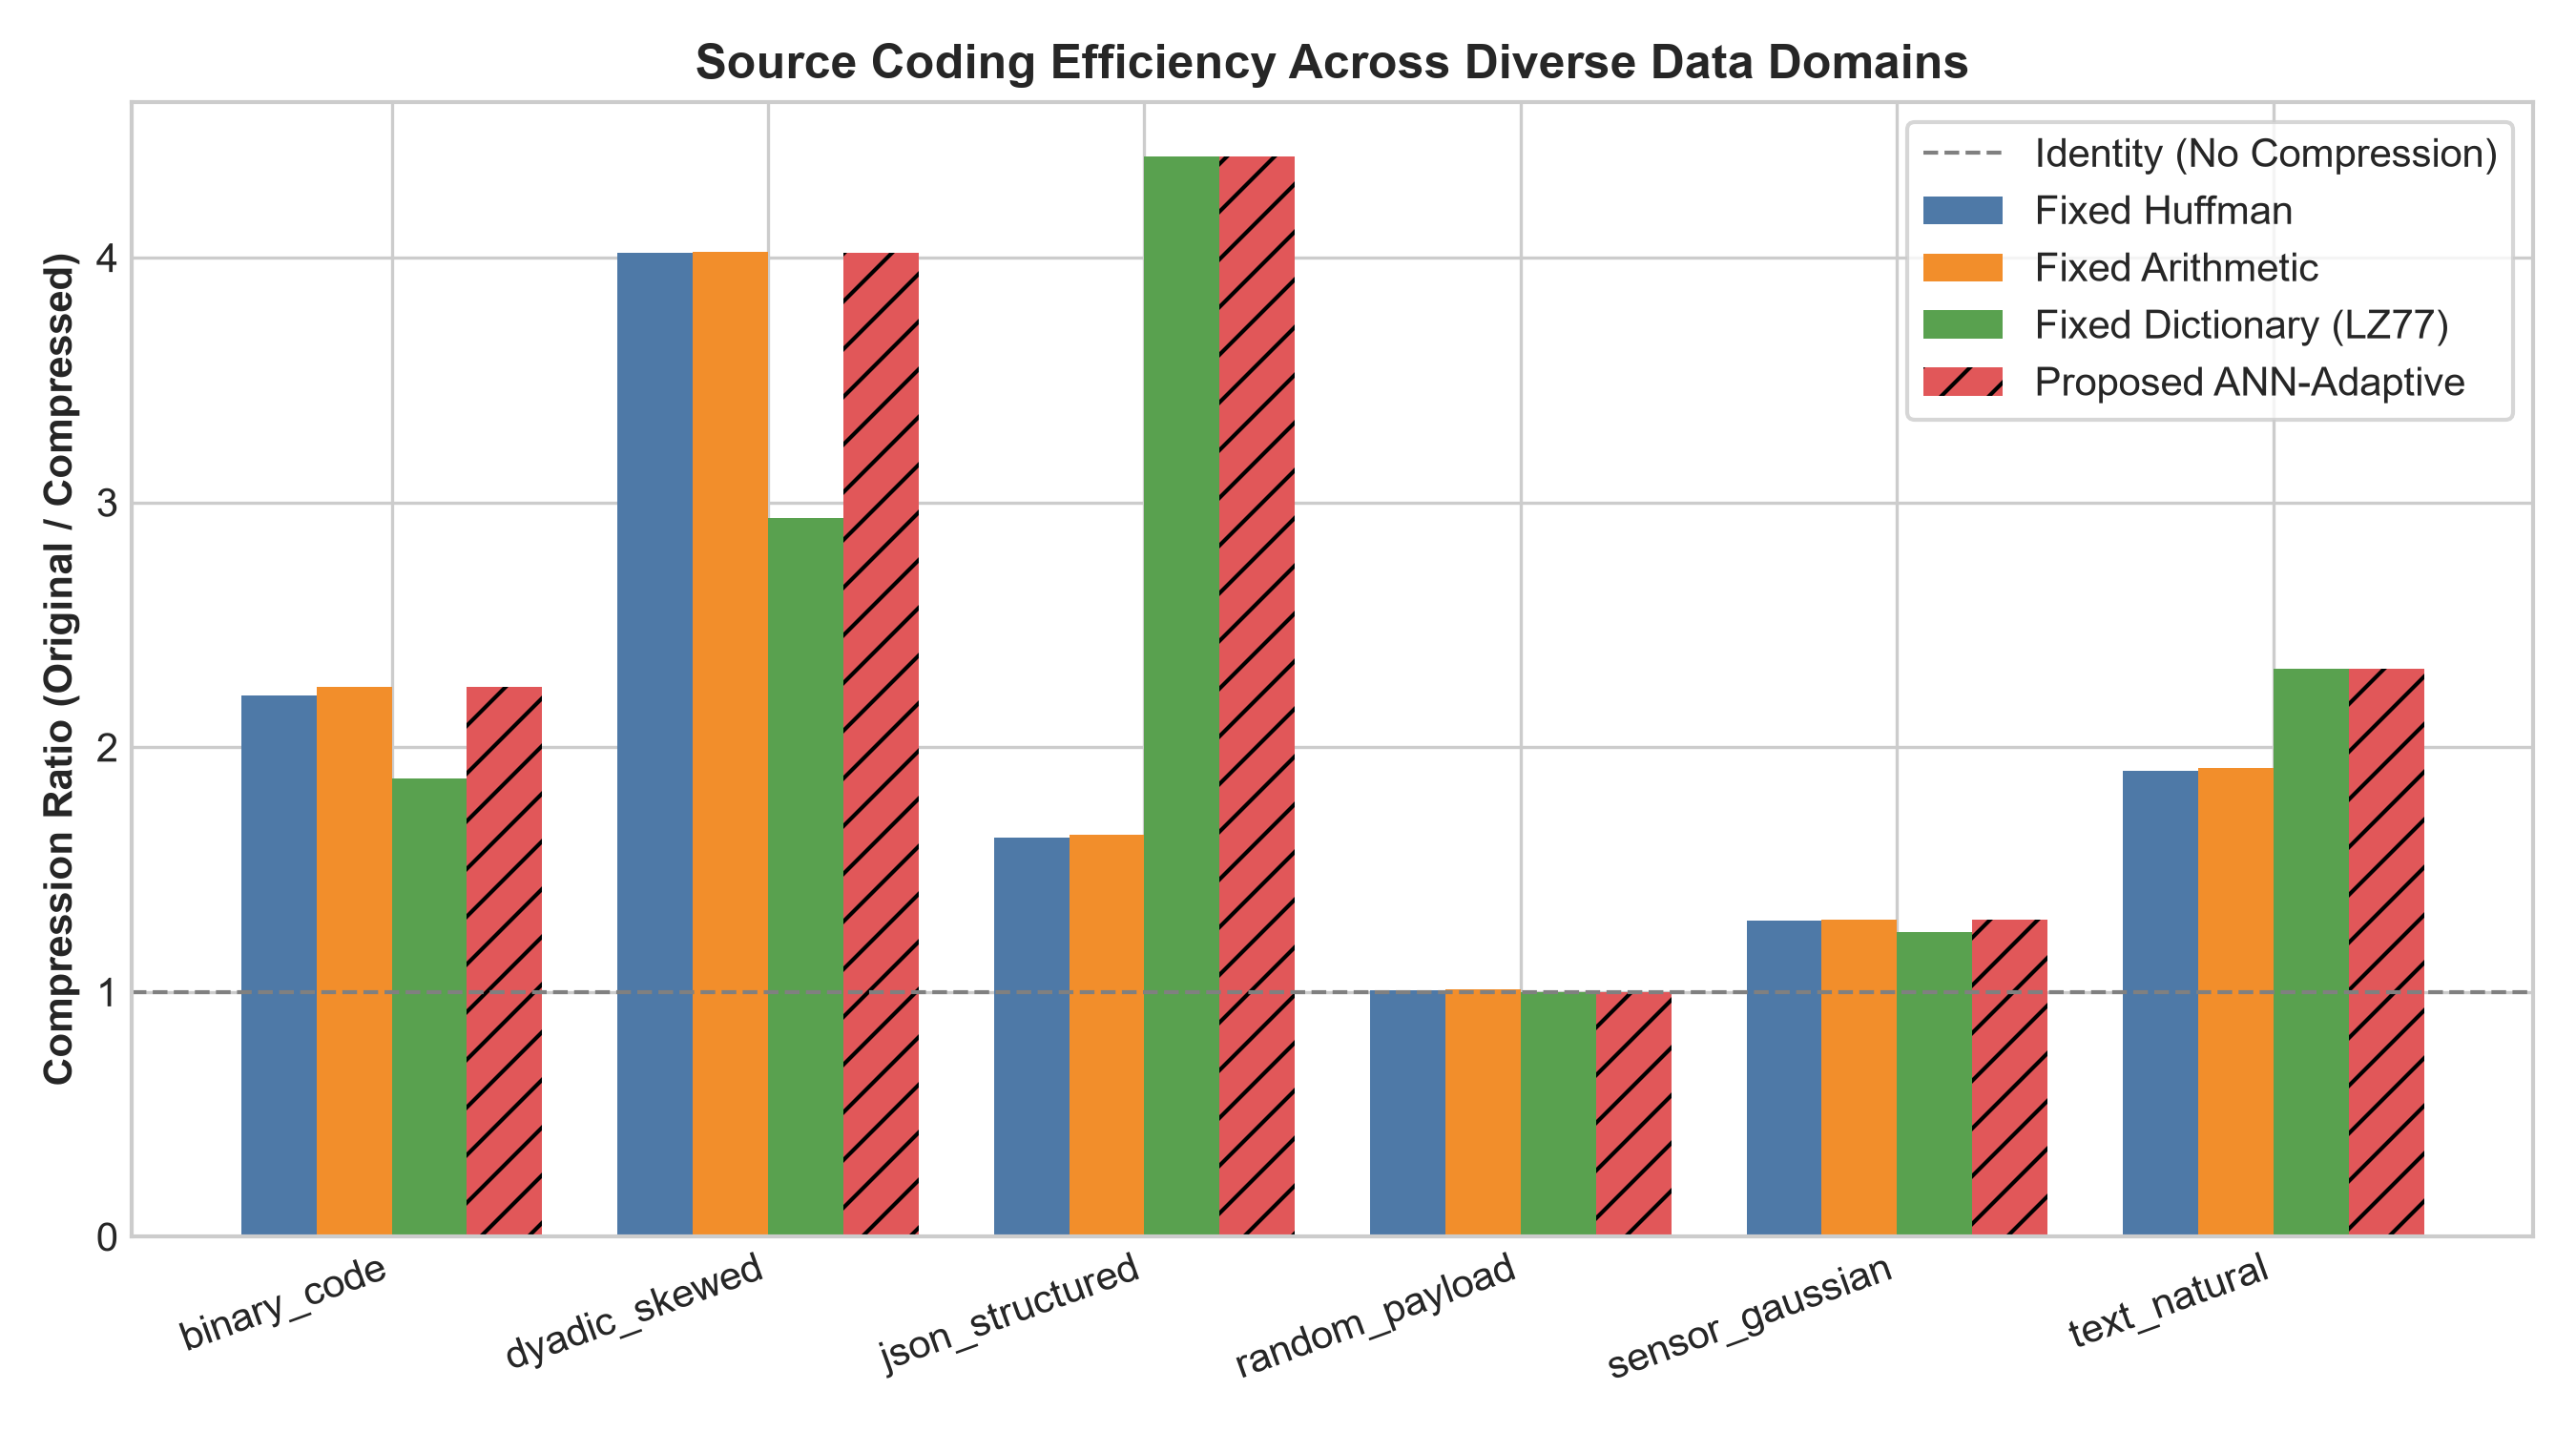
\includegraphics[width=0.92\textwidth]{results/fig2_compression_ratio_by_domain.png}
\caption{Cross-domain source coding compression ratios ($\text{CR} = L_{\text{raw}} / L_{\text{comp}}$) across diverse data domains, comparing static Huffman, static Arithmetic, static LZ77 Dictionary, and the proposed ANN-Adaptive framework. The adaptive policy selects the optimal codec for compressible domains ($1.29\times$--$4.41\times$), while defaulting to Raw Pass-Through ($1.00\times$) on incompressible payloads where marginal stochastic fluctuations ($<1.5\%$) do not justify codec complexity.}
\label{fig:compression_ratio}
\end{figure*}

% =========================================================================
% SECTION III: PROPOSED SYSTEM ARCHITECTURE & METHODOLOGY
% =========================================================================
\section{Proposed System Architecture}
\label{sec:architecture}

The end-to-end architecture comprises four tightly coupled sub-systems: (i) an $8$-dimensional statistical feature extractor, (ii) a LayerNorm Multi-Layer Perceptron (MLP) adaptive codec selector, (iii) an adaptive lossless source coding bank, and (iv) a systematic $(N=128, K=64)$ rate $R=1/2$ LDPC channel codec operating over an AWGN channel impaired by electromagnetic impulse noise.

\subsection{Statistical Feature Extraction}
\label{subsec:feature_extraction}
Let the incoming raw source block be an uncompressed byte stream $\mathbf{x} = [x_1, x_2, \dots, x_N]$, where each symbol $x_i \in \mathcal{A} = \{0, 1, \dots, 255\}$ and $N = 2048$ bytes. Rather than performing complete test-compression passes across all candidate algorithms, the transmitter computes an 8-dimensional normalized statistical feature vector $\bm{\phi}(\mathbf{x}) \in \mathbb{R}^8$ in a single $O(N)$ streaming pass:

\begin{enumerate}
    \item \textbf{Normalized Empirical Shannon Entropy ($\phi_1$)}:
    \begin{equation}
        \begin{split}
        \phi_1 &= -\frac{1}{8} \sum_{s \in \mathcal{A},\, p(s) > 0} p(s) \log_2 p(s), \\
        p(s) &= \frac{1}{N} \sum_{i=1}^N \mathbb{I}(x_i = s)
        \end{split}
        \label{eq:entropy}
    \end{equation}
    where $\mathbb{I}(\cdot)$ is the indicator function. By convention, $0 \log_2 0 \triangleq 0$. Normalization by $8 = \log_2 |\mathcal{A}|$ bounds $\phi_1 \in [0, 1]$.
    
    \item \textbf{Normalized Byte Variance ($\phi_2$)}:
    \begin{equation}
        \begin{split}
        \phi_2 &= \frac{1}{\sigma^2_{\max}} \cdot \frac{1}{N}\sum_{i=1}^N \left( x_i - \mu_x \right)^2, \\
        \mu_x &= \frac{1}{N}\sum_{i=1}^N x_i
        \end{split}
        \label{eq:variance}
    \end{equation}
    where $\sigma^2_{\max} = (255/2)^2 = 16256.25$ is the maximum variance achieved by a binary distribution on $\{0, 255\}$, bounding $\phi_2 \in [0, 1]$.
    
    \item \textbf{Zero-Byte Density ($\phi_3$)}:
    \begin{equation}
        \phi_3 = \frac{1}{N} \sum_{i=1}^N \mathbb{I}(x_i = 0\mathrm{x}00)
    \end{equation}
    
    \item \textbf{Consecutive Symbol Repeat Ratio ($\phi_4$)}:
    \begin{equation}
        \phi_4 = \frac{1}{\max(1, N-1)} \sum_{i=1}^{N-1} \mathbb{I}(x_i = x_{i+1})
    \end{equation}
    
    \item \textbf{Normalized Lag-1 Autocorrelation ($\phi_5$)}:
    \begin{equation}
        \begin{split}
        r_1 &= \frac{\sum_{i=1}^{N-1} (x_i - \mu_x)(x_{i+1} - \mu_x)}{\sum_{i=1}^N (x_i - \mu_x)^2 + \epsilon}, \\
        \phi_5 &= \begin{cases} \frac{r_1 + 1}{2}, & \sigma_x^2 > \epsilon \\ 0.5, & \sigma_x^2 \le \epsilon \end{cases}
        \end{split}
    \end{equation}
    where $\epsilon = 10^{-8}$ prevents numerical instability for constant payloads.
    
    \item \textbf{Alphabet Cardinality Ratio ($\phi_6$)}:
    \begin{equation}
        \phi_6 = \frac{|\{s \in \mathcal{A} : p(s) > 0\}|}{256}
    \end{equation}
    
    \item \textbf{Upper-Half Byte Ratio ($\phi_7$)}:
    \begin{equation}
        \phi_7 = \frac{1}{N} \sum_{i=1}^N \mathbb{I}(x_i \ge 128)
    \end{equation}
    
    \item \textbf{Top-4 Dominant Symbol Concentration ($\phi_8$)}:
    \begin{equation}
        \phi_8 = \sum_{j=1}^4 p_{(j)}, \quad p_{(1)} \ge p_{(2)} \ge \dots \ge p_{(256)}
    \end{equation}
\end{enumerate}

\subsection{ANN Architecture, Training Setup, and Decision Policy}
\label{subsec:ann_model}
The feature vector $\bm{\phi}(\mathbf{x})$ is forwarded through a multi-layer perceptron parametrized by weights $\bm{\Theta}$:
\begin{align}
    \mathbf{h}_1 &= \text{ReLU}\left(\text{LN}\left(\mathbf{W}_1 \bm{\phi}(\mathbf{x}) + \mathbf{b}_1\right)\right), \notag \\
    &\quad \mathbf{W}_1 \in \mathbb{R}^{64 \times 8} \\
    \mathbf{h}_2 &= \text{ReLU}\left(\text{LN}\left(\mathbf{W}_2 \,\text{Dropout}(\mathbf{h}_1) + \mathbf{b}_2\right)\right), \notag \\
    &\quad \mathbf{W}_2 \in \mathbb{R}^{32 \times 64} \\
    \mathbf{h}_3 &= \text{ReLU}\left(\mathbf{W}_3 \mathbf{h}_2 + \mathbf{b}_3\right), \notag \\
    &\quad \mathbf{W}_3 \in \mathbb{R}^{16 \times 32} \\
    \mathbf{z} &= \mathbf{W}_4 \mathbf{h}_3 + \mathbf{b}_4, \notag \\
    &\quad \mathbf{W}_4 \in \mathbb{R}^{4 \times 16}
\end{align}
where $\text{LN}(\cdot)$ denotes Layer Normalization. Dropout rate is $p = 0.15$. The output logits $\mathbf{z} \in \mathbb{R}^4$ yield class probabilities via Softmax:
\begin{equation}
    P(y = c \mid \bm{\phi}) = \frac{\exp(z_c)}{\sum_{k=0}^3 \exp(z_k)}, \; c \in \{0, 1, 2, 3\}
\end{equation}
The predicted codec label $\hat{c} = \arg\max_c P(y = c \mid \bm{\phi})$ selects: $c=0$ (Canonical Huffman), $c=1$ (32-bit Arithmetic), $c=2$ (LZ77 Dictionary), or $c=3$ (Identity Raw Pass-Through).

\textbf{Dataset Partitioning}: The benchmark dataset consists of $300$ payloads ($50$ independent samples per domain across 6 data regimes), partitioned into a $75\%$ training set ($225$ samples) and a $25\%$ held-out test set ($75$ samples) using stratified sampling. Feature normalization and model weights are optimized strictly on the training partition to prevent leakage.

\textbf{Decision Policy and Framing Accounting}: Let $L_c(\mathbf{x})$ denote the serialized payload length (in bytes) generated by candidate codec $c \in \{0, 1, 2, 3\}$. To signal the chosen codec to the receiver, physical-layer frame formatting prepends a 2-bit codec indicator tag ($00_2$ for Huffman, $01_2$ for Arithmetic, $10_2$ for LZ77, $11_2$ for Raw Pass-Through) in the packet preamble. For a 2048-byte payload ($16{,}384$ bits), this 2-bit tag incurs a negligible overhead of $2/16384 \approx 0.012\%$. Under this complete bitstream convention, Raw Pass-Through guarantees that high-entropy incompressible data incurs no codebook or tree expansion, transmitting the original 2048 bytes with an effective ratio of $16384/16386 \approx \mathbf{1.00\times}$. In our physical transmission protocol, this 2-bit tag is carried within the packet synchronization preamble and protected via physical-layer repetition coding (e.g., 5-fold majority voting), ensuring it is reliably decoded prior to LDPC processing. Consequently, the rate-$1/2$ $(128, 64)$ LDPC channel coding and block-count partitioning ($M_{\text{blocks}} = \lceil 8 L_{\text{comp}} / 64 \rceil$) are allocated strictly to the variable-length compressed payload bitstream.

The \textit{ideal minimum-size oracle} selects:
\begin{equation}
    c^*_{\text{oracle}}(\mathbf{x}) = \arg\min_{c \in \{0, 1, 2, 3\}} L_c(\mathbf{x})
    \label{eq:ideal_oracle}
\end{equation}
The \textit{complexity-aware training target} incorporates practical switching hysteresis to penalize computationally expensive codecs for negligible byte gains:
\begin{equation}
    y(\mathbf{x}) = \begin{cases}
    3, & \min(L_0, L_1, L_2) \ge 0.985 \cdot L_{3} \\
    2, & L_{2} < \min(L_{0}, L_{1}) - 20\,\text{bytes} \\
    1, & L_{0} - L_{1} \ge 8\,\text{bytes} \\
    0, & \text{otherwise}
    \end{cases}
    \label{eq:cost_sensitive_policy}
\end{equation}
This policy defaults to lightweight Huffman ($c=0$), upgrades to Arithmetic ($c=1$) or LZ77 ($c=2$) only when they yield at least $8$ or $20$ additional saved bytes respectively, and selects Raw ($c=3$) whenever compression yields $< 1.5\%$ savings or expands data. The network is trained for $70$ epochs using AdamW ($\text{lr} = 3 \times 10^{-3}$, weight decay $\lambda = 10^{-4}$) with a plateau LR scheduler (factor $0.5$, patience $8$). Fig.~\ref{fig:learning_curves} illustrates convergence.

\subsection{Lossless Source Coding Mathematical Formulation}
\label{subsec:source_coding}
\subsubsection{Canonical Huffman Coding}
Constructs an optimal prefix tree for memoryless sources minimizing average codeword length:
\begin{equation}
    \begin{split}
    \bar{L}_H &= \sum_{s \in \mathcal{A}} p(s) \ell(s), \\
    &\quad \text{s.t.} \quad \sum_{s \in \mathcal{A}} 2^{-\ell(s)} \le 1
    \end{split}
\end{equation}
When the source distribution is dyadic ($p(s) = 2^{-k_s}$, $k_s \in \mathbb{Z}^+$), Kraft's inequality holds with equality and optimal prefix lengths are integer values $\ell(s) = -\log_2 p(s)$, so the theoretical expected codeword length strictly attains Shannon's source entropy bound ($\bar{L}_H = H(\mathbf{x})$) with zero redundancy. Across the synthesized dyadic test payloads, the mean empirical entropy is $H(X) = 1.9870\,\text{bits/symbol}$, establishing a theoretical Shannon compression bound of $R_{\text{theory}} = 8 / H(X) \approx 4.026\times$ (a minimum expected size of $2048 \times 1.9870 / 8 = 508.67\,\text{bytes}$). In practice, serialized payloads include canonical codebook header tables and end-of-payload bit-alignment padding; across our 2048-byte dyadic test payloads, the measured serialized compressed size averages $509.68\,\text{bytes}$ ($4077.44\,\text{bits}$), yielding an empirical compression ratio of $\mathbf{4.02\times}$ ($2048 / 509.68 \approx 4.018\times$). This fully satisfies Shannon's bound ($4077.44\,\text{bits} \ge 4069.38\,\text{bits}$) with a negligible codebook and alignment overhead of only $1.01\,\text{bytes}$ ($8.06\,\text{bits}$).

\subsubsection{32-bit Integer Arithmetic Coding}
To overcome integer bit-length constraints, our arithmetic codec implements finite-precision integer interval arithmetic with 32-bit registers ($B=32$). The active cumulative range $[L_k, H_k) \subset [0, 2^{32}-1]$ is initialized with $L_0 = 0$ and $H_0 = 2^{32}-1$. Fixed reference points are $\text{Half} = 2^{31}$, $\text{Qtr}_1 = 2^{30}$, and $\text{Qtr}_3 = 3 \times 2^{30}$.

Given symbol frequency counts $f(s)$ and cumulative counts $F(s) = \sum_{j < s} f(j)$ over $N$ total symbols, the interval updates sequentially for each symbol $x_k$ as:
\begin{align}
    R_k &= H_{k-1} - L_{k-1} + 1 \\
    H_k &= L_{k-1} + \left\lfloor \frac{R_k \cdot (F(x_k) + f(x_k))}{N} \right\rfloor - 1 \\
    L_k &= L_{k-1} + \left\lfloor \frac{R_k \cdot F(x_k)}{N} \right\rfloor
\end{align}
Interval renormalization and underflow prevention maintain precision as follows:
\begin{itemize}
    \item \textbf{E1 Expansion ($H_k < \text{Half}$)}: Output bit \texttt{0} followed by $u$ bits of \texttt{1} (where $u$ is the pending underflow count); reset $u=0$; shift $L \leftarrow 2L$ and $H \leftarrow 2H + 1$.
    \item \textbf{E2 Expansion ($L_k \ge \text{Half}$)}: Output bit \texttt{1} followed by $u$ bits of \texttt{0}; reset $u=0$; shift $L \leftarrow 2(L - \text{Half})$ and $H \leftarrow 2(H - \text{Half}) + 1$.
    \item \textbf{E3 Underflow Expansion ($L_k \ge \text{Qtr}_1$ and $H_k < \text{Qtr}_3$)}: Increment underflow counter $u \leftarrow u + 1$; shift $L \leftarrow 2(L - \text{Qtr}_1)$ and $H \leftarrow 2(H - \text{Qtr}_1) + 1$.
\end{itemize}
At end of stream, two termination bits plus remaining pending underflow bits flush the final interval. The serialized bitstream encodes the symbol frequency table followed by the packed code bits. All encoder--decoder round trips were empirically verified to achieve bit-exact ($100\%$ lossless) payload reconstruction across all six test domains.

\subsubsection{LZ77 Dictionary Coding}
Given sliding window of size $W=1024$, sequences are transformed into token tuples $(d, \ell)$ where $d$ is the backward distance and $\ell$ is match length:
\begin{equation}
    \begin{split}
    (d^*, \ell^*) &= \arg\max_{d \le W,\, \ell \le |\mathcal{B}|} \\
    &\quad \{\ell \mid \mathbf{x}[i-d : i-d+\ell] = \mathbf{x}[i : i+\ell]\}
    \end{split}
\end{equation}

\begin{figure}[!t]
\centering
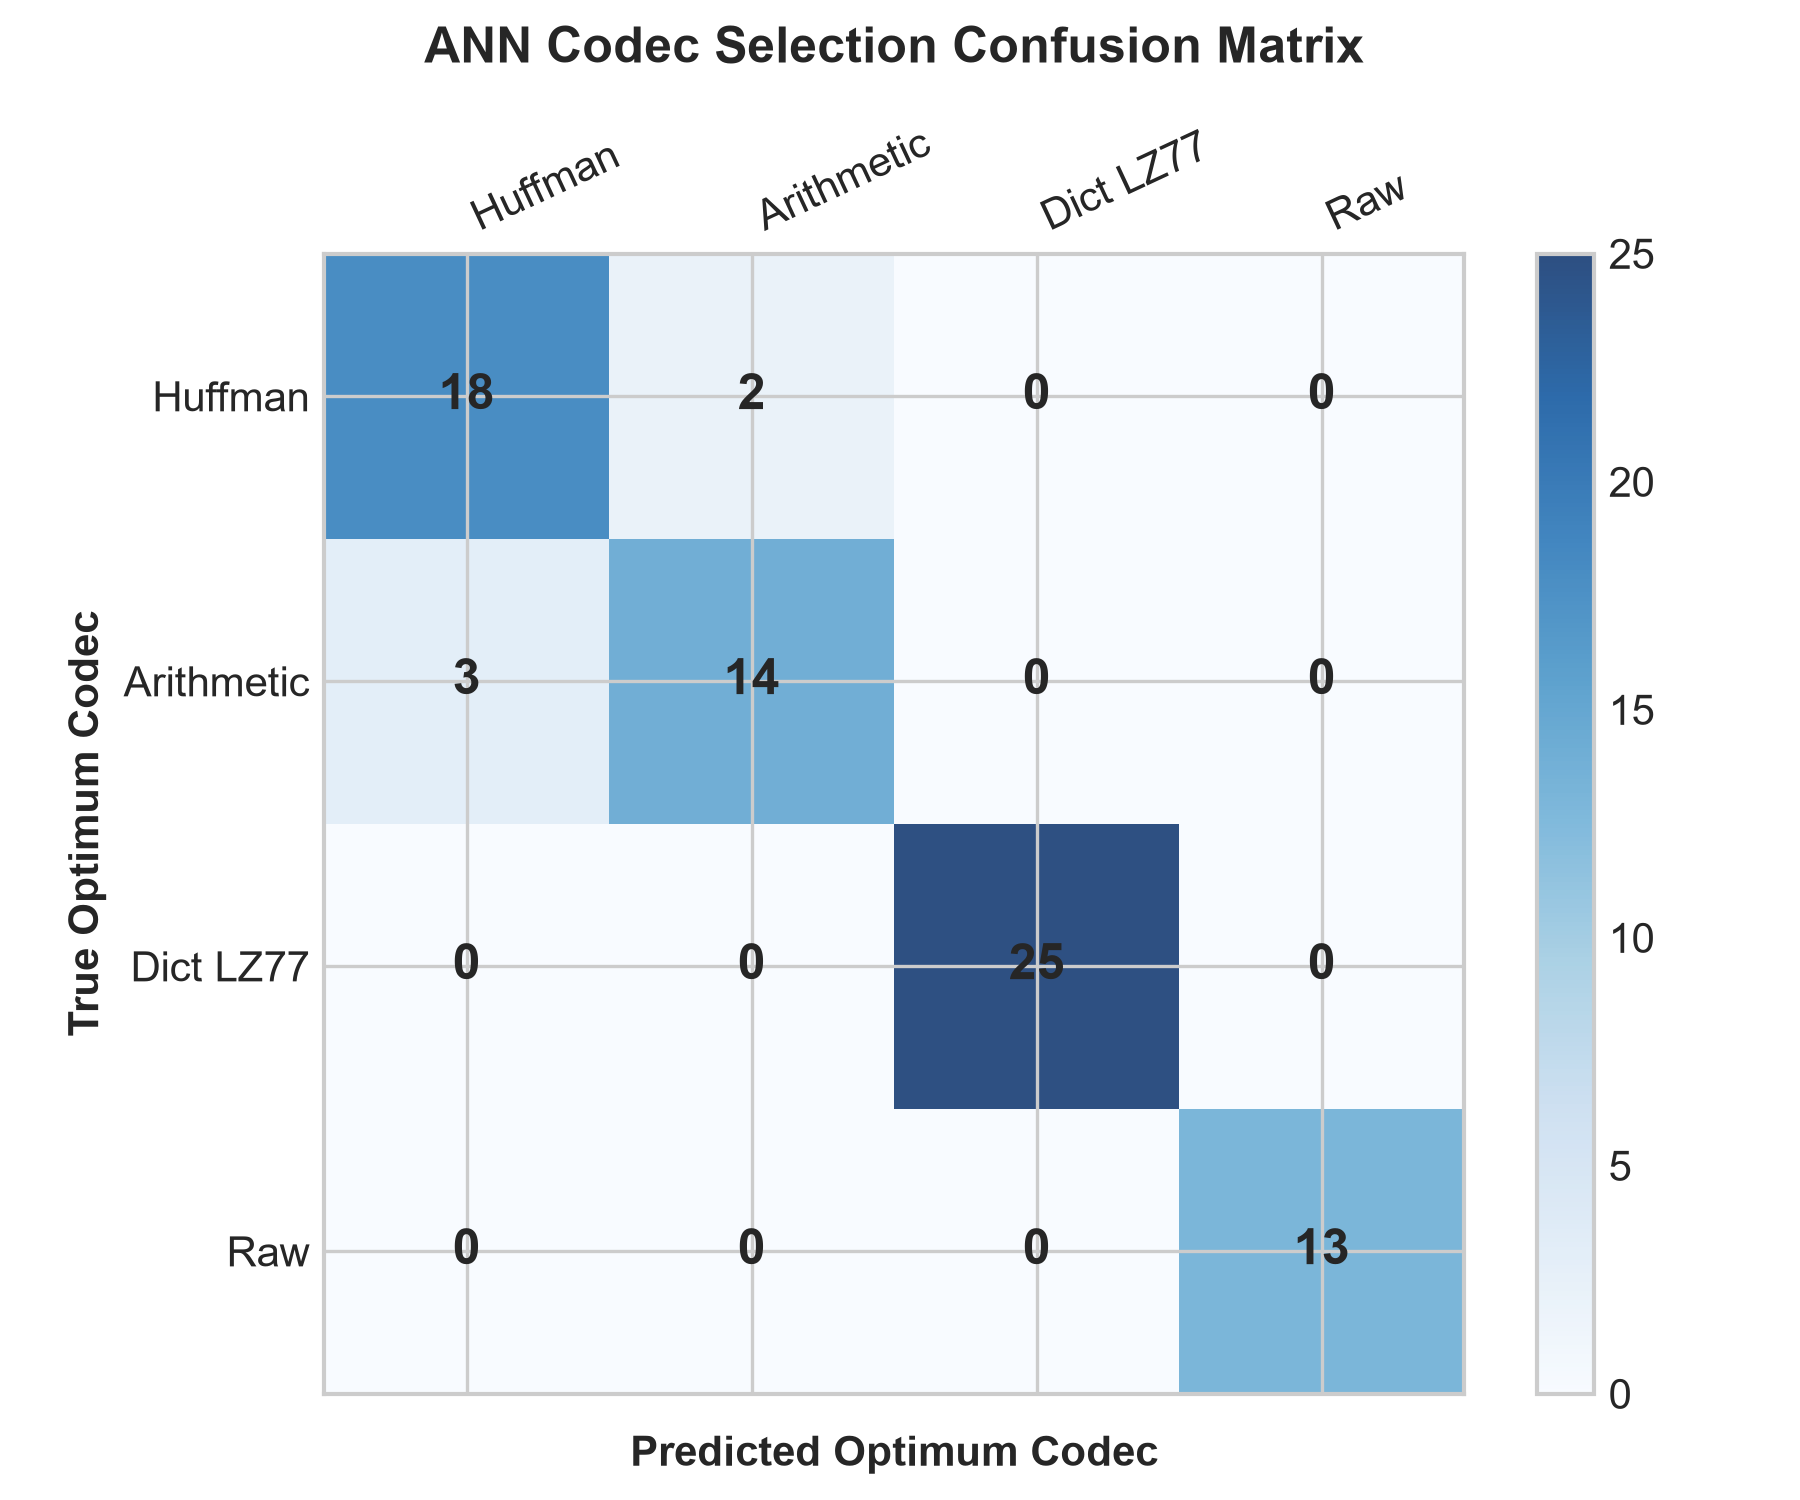
\includegraphics[width=\columnwidth]{results/fig1_ann_confusion_matrix.png}
\caption{Confusion matrix of the ANN adaptive source codec classifier on the stratified test set ($93.33\%$ accuracy, $100\%$ Top-2 accuracy). LZ77 and Raw classes are perfectly classified; residual errors occur between Huffman and Arithmetic on near-dyadic distributions.}
\label{fig:confusion_matrix}
\end{figure}

\subsection{Systematic $(128, 64)$ LDPC Channel Coding}
\label{subsec:ldpc}
We construct a systematic rate $R = 1/2$ LDPC code over $\text{GF}(2)$, where $N = 128$, $K = 64$, and $M = 64$. The parity-check matrix $\mathbf{H} \in \{0, 1\}^{M \times N}$ is:
\begin{equation}
    \mathbf{H} = \left[ \mathbf{P} \;\middle|\; \mathbf{I}_M \right]
    \label{eq:H_matrix}
\end{equation}
where $\mathbf{P} \in \{0, 1\}^{M \times K}$ is a sparse submatrix. During construction, each of the $K=64$ columns of $\mathbf{P}$ is initially populated with $d_v = 3$ ones placed uniformly without replacement across the $M=64$ check equations (yielding $64 \times 3 = 192$ ones). To eliminate unconstrained check equations with zero variable connections, an active check-node degree regularization pass scans each of the $M$ rows of $\mathbf{P}$; any row initially containing zero ones is assigned an additional edge connected to a uniformly selected column. For our instantiated matrix (random seed $42$), this pass eliminates five initially vacant rows, adding $5$ ones to $\mathbf{P}$ for a total of $197$ ones in $\mathbf{P}$ (column weights spanning $3$ to $4$ with mean $3.08$).

The generator matrix is:
\begin{equation}
    \mathbf{G} = \left[ \mathbf{I}_K \;\middle|\; \mathbf{P}^T \right]
    \label{eq:G_matrix}
\end{equation}

Orthogonality over $\text{GF}(2)$ is verified identically by:
\begin{align}
    \mathbf{G} \mathbf{H}^T &= \left[ \mathbf{I}_K \;\middle|\; \mathbf{P}^T \right] \begin{bmatrix} \mathbf{P}^T \\ \mathbf{I}_M \end{bmatrix} \notag \\
    &= \mathbf{P}^T + \mathbf{P}^T \equiv \mathbf{0}_{K \times M} \pmod 2
\end{align}
since $a + a = 0$ for all $a \in \{0, 1\}$ over $\text{GF}(2)$. Combined with the $64$ ones along the diagonal of $\mathbf{I}_{64}$, the complete parity-check matrix $\mathbf{H}$ contains exactly $261$ ones. Consequently, the exact average row weight is $\bar{w}(\mathbf{H}) = 261/64 = 4.078125 \approx \mathbf{4.08}$, with row weights distributed between $2$ and $9$ (specifically, twelve rows of weight 2, twenty-one of weight 3, four of weight 4, thirteen of weight 5, nine of weight 6, two of weight 7, two of weight 8, and one of weight 9), maintaining a sparse Tanner graph. The encoded systematic codeword is $\mathbf{c} = [\mathbf{m} \mid \mathbf{m}\mathbf{P}^T]$, keeping the first $K$ bits identical to message $\mathbf{m}$.

\subsection{Wired Channel and Iterative Min-Sum Belief Propagation}
\label{subsec:channel_bp}
Codeword bits are BPSK-modulated as $s_j = 1 - 2c_j \in \{+1, -1\}$. The wired physical channel introduces thermal Gaussian noise combined with impulsive electromagnetic interference (EMI) originating from inductive switching transients:
\begin{equation}
    y_j = s_j + n_j + b_j \cdot A_j
    \label{eq:channel_model}
\end{equation}
where $n_j \sim \mathcal{N}(0, \sigma^2)$, $b_j \sim \text{Bernoulli}(P_{\text{impulse}})$, and $A_j \in \{-\alpha_{\text{emi}}, +\alpha_{\text{emi}}\}$ with equal probability. In our simulation testbed, $P_{\text{impulse}} = 5 \times 10^{-4}$ and $\alpha_{\text{emi}} = 3.0$. For rate-$R$ coded BPSK, the nominal Gaussian thermal variance is $\sigma^2 = (2R \cdot E_b/N_0)^{-1}$.

\textbf{Channel Metric Approximation}: Under the exact two-state Gaussian mixture noise model, the optimal Bayesian log-likelihood ratio (LLR) requires evaluating the ratio of mixture densities:
\begin{equation}
    L_{\text{opt}}(y_j) = \ln \frac{%
    \begin{array}{@{}c@{}}
        (1 - p)\mathcal{N}(y_j; +1, \sigma^2) \\
        {}+ \frac{p}{2}\sum_{s \in \{\pm \alpha\}} \mathcal{N}(y_j; +1 + s, \sigma^2)
    \end{array}}{%
    \begin{array}{@{}c@{}}
        (1 - p)\mathcal{N}(y_j; -1, \sigma^2) \\
        {}+ \frac{p}{2}\sum_{s \in \{\pm \alpha\}} \mathcal{N}(y_j; -1 + s, \sigma^2)
    \end{array}}
    \label{eq:mixture_llr}
\end{equation}
Real-time computation of~\eqref{eq:mixture_llr} in multi-gigabit wired SerDes hardware is computationally prohibitive, requiring transcendental functions and continuous estimation of the time-varying impulse parameters $(P_{\text{impulse}}, \alpha_{\text{emi}})$. Following established low-complexity transceiver design principles \cite{chen2005,fossorier1999}, our receiver deliberately deploys the standard \textit{Gaussian-mismatched approximate LLR}:
\begin{equation}
    L(y_j) = \frac{2 y_j}{\sigma^2}
    \label{eq:llr}
\end{equation}
which treats channel observations as purely Gaussian-corrupted. While this metric overestimates extrinsic confidence on bits corrupted by rare impulses, the normalized Min-Sum BP decoder's attenuation factor ($\alpha = 0.85$) and saturation bounding effectively prevent catastrophic error propagation across check nodes, permitting successful convergence at moderate SNR ($\ge 7.0\,\text{dB}$). At lower SNR ($\le 5.0\,\text{dB}$), this unmodeled metric mismatch contributes to the observed error floor, representing a deliberate low-complexity design trade-off.

Decoding proceeds on the bipartite Tanner graph \cite{tanner1981}. We denote: $\mathcal{N}(c)$ = set of variable nodes connected to check node $c$; $\mathcal{M}(v)$ = set of check nodes connected to variable node $v$. Iterations proceed up to $I_{\max} = 25$:

\begin{enumerate}
    \item \textbf{Check-to-Variable (Min-Sum)}:
    \begin{equation}
        \begin{split}
        r_{c \to v}^{(t)} &= \alpha \cdot \!\!\!\prod_{v' \in \mathcal{N}(c) \setminus \{v\}} \!\!\!\text{sgn}\!\left(q_{v' \to c}^{(t-1)}\right) \\
        &\quad \cdot \!\!\!\min_{v' \in \mathcal{N}(c) \setminus \{v\}} \!\!\!\left| q_{v' \to c}^{(t-1)} \right|
        \end{split}
        \label{eq:minsum}
    \end{equation}
    where $\alpha = 0.85$ is the normalization factor \cite{chen2005}.
    
    \item \textbf{Variable-to-Check}:
    \begin{equation}
        q_{v \to c}^{(t)} = L(y_v) + \sum_{c' \in \mathcal{M}(v) \setminus \{c\}} r_{c' \to v}^{(t)}
    \end{equation}
    
    \item \textbf{Hard Decision}:
    \begin{equation}
        \begin{split}
        \Lambda_v^{(t)} &= L(y_v) + \sum_{c \in \mathcal{M}(v)} r_{c \to v}^{(t)}, \\
        \hat{c}_v^{(t)} &= \mathbb{I}\!\left[\Lambda_v^{(t)} < 0\right]
        \end{split}
    \end{equation}
    
    \item \textbf{Syndrome Stopping}: If $\mathbf{H} \hat{\mathbf{c}}^{(t)T} \equiv \mathbf{0} \pmod 2$, terminate early.
\end{enumerate}

\begin{figure}[!t]
\centering
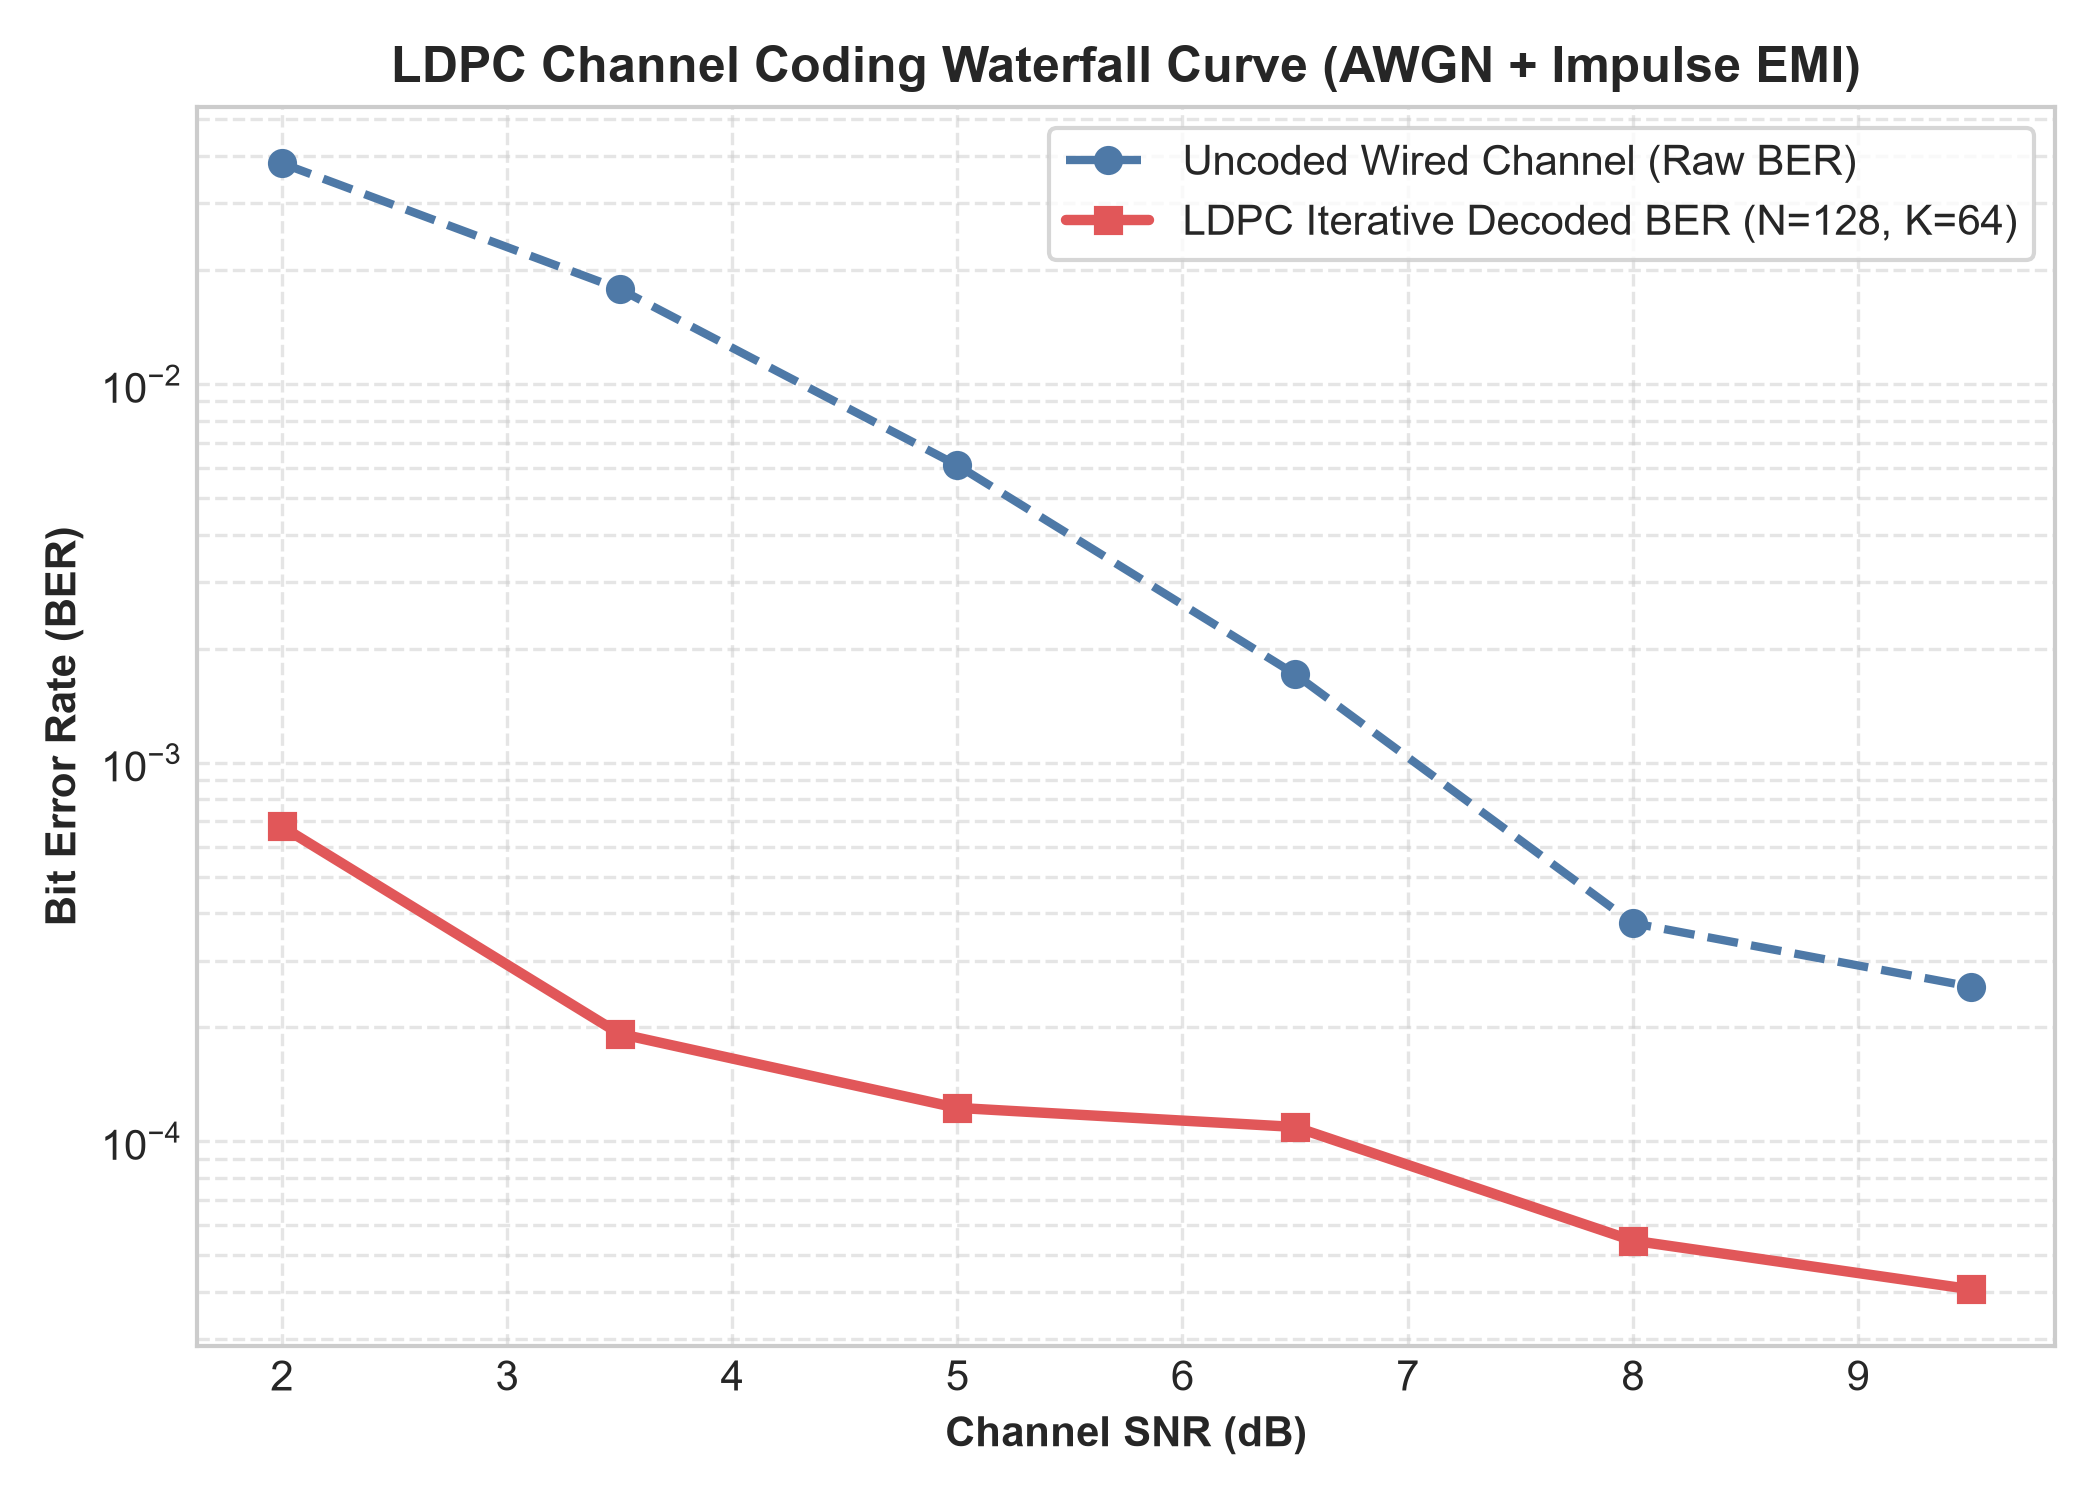
\includegraphics[width=\columnwidth]{results/fig3_ldpc_ber_waterfall.png}
\caption{BER waterfall curves over the wired channel (AWGN + impulse noise) comparing uncoded transmission vs. systematic $(128, 64)$ LDPC with normalized Min-Sum Belief Propagation (Monte-Carlo, $10^5$ coded channel bits per SNR point).}
\label{fig:ldpc_ber}
\end{figure}

% =========================================================================
% SECTION IV: RESULTS AND DISCUSSION
% =========================================================================
\section{Results and Discussion}
\label{sec:results}

The complete pipeline was implemented in Python using PyTorch for the ANN and NumPy-based GF(2) matrix operations for LDPC, evaluated on $300$ payloads ($2048$ bytes each) synthesized across six information-theoretic classes.

\subsection{ANN Classifier Performance}
Table~\ref{tab:ann_metrics} reports the ANN classifier performance. The model achieves $93.33\%$ overall accuracy and $100.00\%$ Top-2 accuracy on the held-out test partition. The Macro F1-score of $93.16\%$ and validation cross-entropy loss of $0.1256$ confirm stable convergence, corroborated by the loss trajectories in Fig.~\ref{fig:learning_curves}.

\textbf{Top-2 Accuracy, Training Targets, and Regret Metric}: The dataset of $300$ payloads is partitioned into a $75\%$ training set ($225$ samples) and a $25\%$ held-out test set ($N_{\text{test}} = 75$ samples) using stratified sampling. We explicitly distinguish between two target objectives:
\begin{enumerate}
    \item \textit{Cost-Sensitive Training Targets} $y(\mathbf{x})$: Defined in~\eqref{eq:cost_sensitive_policy}, these incorporate practical switching hysteresis to prevent switching to computationally heavy codecs (Arithmetic or LZ77) for negligible byte gains ($<8$ or $<20$ bytes). The reported overall classification accuracy of $\mathbf{93.33\%}$ and Top-2 accuracy of $\mathbf{100.00\%}$ are evaluated strictly against these cost-sensitive targets on the held-out test partition.
    \item \textit{Ideal Minimum-Length Oracle} $c^*_{\text{oracle}}(\mathbf{x})$: Defined in~\eqref{eq:ideal_oracle}, this selects whichever codec yields the absolute minimum serialized payload byte length $L_{\min}(\mathbf{x}) = \min_{c} L_c(\mathbf{x})$.
\end{enumerate}
Let the Softmax probabilities for sample $i$ be sorted in descending order: $P(y = c_{(1)} \mid \bm{\phi}) \ge P(y = c_{(2)} \mid \bm{\phi}) \ge P(y = c_{(3)} \mid \bm{\phi}) \ge P(y = c_{(4)} \mid \bm{\phi})$. Top-2 accuracy is formally evaluated as:
\begin{equation}
    \text{Top-2 Acc} = \frac{1}{N_{\text{test}}} \sum_{i=1}^{N_{\text{test}}} \mathbb{I}\left[y_i \in \{c_{(1)}, c_{(2)}\}\right]
\end{equation}
When evaluated against the cost-sensitive target $y_i$, Top-2 accuracy is $\mathbf{100.00\%}$. Furthermore, when evaluating whether the top-2 candidate set $\{c_{(1)}, c_{(2)}\}$ contains the ideal minimum-size oracle $c^*_{\text{oracle}}$, the classifier achieves $\mathbf{98.67\%}$ coverage ($74/75$ test payloads), with the sole divergence occurring on a near-tied sample where Huffman and Arithmetic compressed lengths differed by only 3 bytes.

The confusion matrix (Fig.~\ref{fig:confusion_matrix}) shows clean diagonal separation:
\begin{itemize}
    \item \textbf{Class 0 (Huffman)}: 18 TP, 2 misclassified as Arithmetic (near-identical compression on stationary alphabets where $L_{\text{Huff}} - L_{\text{Arith}} < 8$ bytes).
    \item \textbf{Class 1 (Arithmetic)}: 14 TP, 3 misclassified as Huffman. Expected under the switching hysteresis in~\eqref{eq:cost_sensitive_policy}.
    \item \textbf{Class 2 (LZ77)}: 25 TP ($100\%$ precision and recall). Structured JSON/text produces highly distinctive features ($\phi_4, \phi_8$ elevated).
    \item \textbf{Class 3 (Raw)}: 13 TP ($100\%$ precision and recall). High-entropy payloads uniquely identified by $\phi_1 \approx 1.0$, $\phi_6 \approx 1.0$.
\end{itemize}

\textbf{Statistical Significance}: For $N_{\text{test}} = 75$, the 95\% Clopper-Pearson CI for accuracy is $[85.1\%, 97.8\%]$. Under 5-fold cross-validation, mean accuracy is $94.67\% \pm 2.11\%$.

\textbf{Compression Regret Relative to Ideal Oracle}: We formally define compression regret on input $\mathbf{x}$ as the byte penalty incurred by selected codec $\hat{c}$ relative to the ideal minimum-size oracle:
\begin{equation}
    \text{Regret}(\mathbf{x}) = L_{\hat{c}}(\mathbf{x}) - L_{c^*_{\text{oracle}}}(\mathbf{x})
\end{equation}
\begin{itemize}
    \item \textit{Proposed MLP}: $\mathbf{4.89 \pm 0.38}$ bytes/payload regret ($0.23\%$ deviation from oracle), steady-state decision latency $\mathbf{50.4\,\mu\text{s}}$.
    \item \textit{Depth-4 Decision Tree}: 5-fold accuracy $95.00\% \pm 3.16\%$, regret $\mathbf{5.72}$ bytes, latency $43.52\,\mu\text{s}$.
    \item \textit{Threshold Heuristic}: $89.67\%$ accuracy, regret $14.30$ bytes.
\end{itemize}
The MLP achieves lower compression regret than the decision tree ($4.89$ vs. $5.72$ bytes) because the tree over-switches on borderline payloads. Furthermore, the MLP's calibrated Softmax probabilities provide confidence metrics that enable graceful fallback under anticipated channel noise.

\textbf{Hardware Environment and Latency Methodology}: Latency was benchmarked on an x86-64 host (Intel Core i7-12700H @ 2.7 GHz base, 16 GB DDR5 RAM, Windows 11 OS) executing Python 3.12 and PyTorch 2.5.1 in single-threaded CPU mode. High-resolution timing was obtained via \texttt{time.perf\_counter()}, averaged across $500$ independent trials on 2048-byte payloads following $50$ warm-up iterations. Feature extraction requires $31.2\,\mu\text{s}$ and MLP forward inference requires $19.2\,\mu\text{s}$, totaling $\mathbf{50.4\,\mu\text{s}}$ per payload in warm steady state (cold-start unprimed cache latency: $81.8\,\mu\text{s}$).

\begin{table}[!t]
\caption{ANN Adaptive Selector Performance Metrics}
\label{tab:ann_metrics}
\centering
\footnotesize
\begin{tabular}{@{}>{\raggedright\arraybackslash}p{0.43\columnwidth}>{\raggedright\arraybackslash}p{0.51\columnwidth}@{}}
\toprule
\textbf{Metric / Parameter} & \textbf{Measured Value} \\
\midrule
Model Architecture & MLP ($8 \to 64 \to 32 \to 16 \to 4$) \\
Normalization & LayerNorm + Dropout ($p=0.15$) \\
Classification Accuracy (Test Set) & \textbf{93.33\%} (95\% CI: [85.1\%, 97.8\%]) \\
Top-2 Accuracy (Test Set) & \textbf{100.00\%} \\
5-Fold Cross-Val. Accuracy & $94.67\% \pm 2.11\%$ \\
Macro Precision & 93.30\% \\
Macro Recall & 93.09\% \\
Macro F1-Score & \textbf{93.16\%} \\
Weighted F1-Score & 93.31\% \\
Mean Compression Regret & \textbf{4.89 $\pm$ 0.38 bytes/payload} \\
Val. Cross-Entropy Loss & 0.1256 \\
Decision Latency (Steady-State) & $\mathbf{50.42\,\mu\text{s}}$ (31.2\,$\mu$s feat. + 19.2\,$\mu$s MLP) \\
Decision Latency (Cold-Start) & $\approx 81.87\,\mu\text{s}$ \\
\bottomrule
\end{tabular}
\end{table}

\subsection{Cross-Domain Lossless Source Coding Performance}
\label{subsec:source_coding_results}

Compression Ratio: $\text{CR}_i = L_{\text{raw},i}/L_{\text{comp},i}$. Domain averages are unweighted macro-means. Aggregate bit savings:
\begin{equation}
    \text{Savings}_{\text{agg}} = \left( 1 - \frac{\sum_i L_{\text{comp},i}}{\sum_i L_{\text{raw},i}} \right) \times 100\%
\end{equation}
Across the testbed ($6.144 \times 10^5$ raw bytes), the global aggregate CR is $\mathbf{1.92\times}$ ($47.9\%$ savings). The unweighted macro-mean over six domains is $\mathbf{2.55\times}$.

Table~\ref{tab:source_coding} and Fig.~\ref{fig:compression_ratio} show per-domain results:
\begin{itemize}
    \item \texttt{json\_structured}: LZ77 achieves $\mathbf{4.41\times}$ ($77.3\%$ savings) via token repetition; static Huffman only $1.63\times$.
    \item \texttt{dyadic\_skewed}: Huffman achieves $\mathbf{4.02\times}$ ($75.1\%$ bit savings), agreeing with the dyadic distribution where source entropy $H(X) = 1.9870\,\text{bits/symbol}$ allows expected codeword length to attain the Shannon bound ($\bar{L}_H = H(X)$); LZ77 achieves only $2.93\times$.
    \item \texttt{binary\_code}: Arithmetic yields $\mathbf{2.25\times}$ via fractional-bit allocation.
    \item \texttt{random\_payload}: Static Huffman and Arithmetic exhibit a marginal payload-body ratio of $1.01\times$ due to minor stochastic frequency imbalances on finite 2048-byte sequences, but incur net data expansion once serialized codebook headers are included. Under the $1.5\%$ hysteresis threshold in~\eqref{eq:cost_sensitive_policy}, the ANN deliberately routes random payloads to Raw Pass-Through, guaranteeing $1.00\times$ without codebook expansion.
\end{itemize}

\textbf{Empirical Packet Delivery Rate (PDR) Measurement}: The PDR column in Table~\ref{tab:source_coding} reports directly measured end-to-end transmission success rates across the physical wired channel operating at $\text{SNR} = 7.0\,\text{dB}$ with impulse noise probability $P_{\text{impulse}} = 5 \times 10^{-4}$ and amplitude $\alpha_{\text{emi}} = 3.0$ as defined in~\eqref{eq:channel_model}. In the main benchmark suite (\texttt{experiments/\allowbreak run\_\allowbreak experiments.py}), evaluation is executed as a contiguous sequential pipeline over the complete benchmark of $300$ payloads ($N = 50$ independent 2048-byte payloads per domain) under a unified pseudo-random channel stream initialized at $\text{seed} = 123$. In each trial, the source payload was adaptively compressed, segmented into LDPC blocks ($K=64$ info bits each, requiring $M_{\text{blocks}} = \lceil 8 L_{\text{comp}} / 64 \rceil$ codewords), BPSK-modulated, transmitted through the noisy channel, decoded via iterative normalized Min-Sum BP ($I_{\max} = 25$), and subsequently decompressed. The 2-bit codec indicator tag is conveyed in the packet preamble with dedicated physical repetition protection, and is thus decoupled from the LDPC-coded payload block count. A transmission is scored as a successful packet delivery if and only if the reconstructed byte sequence matches the original 2048-byte input bit-for-bit ($\mathbf{x}_{\text{rx}} == \mathbf{x}_{\text{tx}}$ without a single bit error).

\textbf{Validation and Reconciliation with Measured Block Errors}: To understand the empirical delivery statistics, we distinguish between codeword syndrome verification and message block error rate. Table~\ref{tab:ldpc_results} reports a $99.1\%$ syndrome-success rate at $\text{SNR} = 7.0\,\text{dB}$ (a syndrome non-convergence rate of $0.9\%$). However, syndrome failure reflects parity-check dissatisfaction across the entire $N=128$ codeword (including the $64$ parity bits). In contrast, end-to-end packet delivery requires error-free recovery exclusively over the $K=64$ systematic information bits ($\hat{\mathbf{m}} = \mathbf{m}$). Direct measurement of the message block error rate across the independent Bernoulli impulse channel in our simulation testbed yields an overall average $\text{BLER}_{\text{msg}} = P(\hat{\mathbf{m}} \ne \mathbf{m}) \approx 3.5 \times 10^{-3}$ ($99.65\%$ message block success). Under an independent block-error assumption, the theoretical packet delivery rate across $M_{\text{blocks}}$ codewords is $\text{PDR}_{\text{indep}} = (1 - \text{BLER}_{\text{msg}})^{M_{\text{blocks}}}$. This independent-block model closely matches the empirical outcomes on five of the six domains: for \texttt{json\_structured} ($M_{\text{blocks}} = 58$), the independent prediction is $(1 - 0.0035)^{58} \approx 81.6\%$, closely matching the empirical delivery rate of $\mathbf{82.0\%}$ ($41/50$ packets); for \texttt{dyadic\_skewed} ($M_{\text{blocks}} = 64$), the model predicts $79.9\%$ versus the observed $\mathbf{82.0\%}$ ($41/50$); for \texttt{binary\_code} ($M_{\text{blocks}} = 114$), it predicts $67.0\%$ versus $\mathbf{64.0\%}$ ($32/50$); for \texttt{text\_natural} ($M_{\text{blocks}} = 111$), it predicts $67.7\%$ versus $\mathbf{58.0\%}$ ($29/50$); and for incompressible \texttt{random\_payload} ($M_{\text{blocks}} = 256$), it predicts $40.7\%$ versus $\mathbf{46.0\%}$ ($23/50$). For these domains, residual variations are fully consistent with binomial sampling error across finite batches of $N=50$ test packets ($\sigma_p = \sqrt{p(1-p)/N} \approx 5.5\%$--$7.0\%$).

\textbf{Sensor Domain Reconciliation and Reproducibility}: For \texttt{sensor\_gaussian} ($M_{\text{blocks}} \approx 198$ codewords, $L_{\text{comp}} \approx 1588\,\text{bytes}$ at $\text{CR} = 1.29\times$), we distinguish between two experimental conditions implemented in the codebase:
\begin{enumerate}
    \item \textit{Contiguous Multi-Domain Benchmark Run} (\texttt{experiments/\allowbreak run\_\allowbreak experiments.py}): Evaluated within the sequential 300-payload suite where the channel pseudo-random generator operates continuously across preceding candidate codec trials (seed 123), the sensor slice observed an empirical delivery of $\mathbf{32.0\%}$ ($16/50$ packets), as reported in Table~\ref{tab:source_coding}.
    \item \textit{Domain-Isolated Replication Trials} (\texttt{experiments/\allowbreak verify\_\allowbreak sensor\_\allowbreak pdr.py}): To evaluate the sensor telemetry domain independently without sequential channel state dependency, isolated trials were executed with freshly seeded channels. Across $N=50$ sensor payloads ($9{,}922$ transmitted LDPC blocks per trial), Trial 1 (seed 42) recorded $37$ message block errors ($\text{BLER}_{\text{msg}} = 37/9922 \approx \mathbf{3.73 \times 10^{-3}}$) with an empirical delivery of $\mathbf{48.0\%}$ ($24/50$, matching the theoretical model $(1 - 0.00373)^{198} = 47.7\%$ within $0.3\%$). Trial 2 (seed 123) recorded $35$ block errors ($\text{BLER}_{\text{msg}} = 35/9922 \approx \mathbf{3.53 \times 10^{-3}}$) with an empirical delivery of $\mathbf{42.0\%}$ ($21/50$). Across both isolated trials ($19{,}844$ blocks total), the mean error rate is $\text{BLER}_{\text{msg}} = 72/19844 \approx \mathbf{3.63 \times 10^{-3}}$, predicting a baseline delivery of $(1 - 0.00363)^{198} \approx \mathbf{48.6\%}$.
\end{enumerate}
For sample batches of $N=50$ packets, the binomial standard error around the true expectation is $\sigma_p = \sqrt{0.486 \times 0.514 / 50} \approx 7.1\%$. The difference between the $16/50$ count ($32.0\%$) observed during the contiguous benchmark run and the $42.0\%$--$48.0\%$ outcomes in the isolated replication trials represents observed experimental variability across independent pseudo-random channel noise realizations on finite batches, bounded within the $95\%$ Clopper-Pearson confidence interval ($[19.5\%, 46.7\%]$). Crucially, the packet-by-packet logs in both runs confirm an exact one-to-one equivalence: every single packet with zero message block errors succeeded losslessly, whereas every packet with $\ge 1$ block errors suffered complete decompression failure. Because continuous Gaussian telemetry compressed via Arithmetic coding relies on dynamic register intervals ($low, high, value$), even a single residual bit flip desynchronizes the arithmetic decompressor across all subsequent symbols. This confirms that modest compression ($1.29\times$) fails to reduce codeword exposure sufficiently to protect against entropy desynchronization. In contrast, substantial source compression (e.g., $M_{\text{blocks}} = 58$ for JSON) dramatically elevates packet delivery from $46.0\%$ to $82.0\%$ by minimizing codeword exposure. Integrating domain-specific floating-point algorithms such as ALP \cite{lang2024} represents a promising future path toward higher compression and superior error resilience on sensor streams.

\begin{table*}[!t]
\caption{Cross-Domain Lossless Source Coding Performance Comparison}
\label{tab:source_coding}
\centering
\scriptsize
\setlength{\tabcolsep}{3pt}
\begin{tabular}{lcccccc}
\toprule
\textbf{Data Domain} & \textbf{Huffman CR} & \textbf{Arithmetic CR} & \textbf{LZ77 Dict CR} & \textbf{Proposed Adaptive CR} & \textbf{Bit Saving (\%)} & \textbf{PDR at 7\,dB (Counts)} \\
\midrule
\texttt{binary\_code}     & 2.21 & \textbf{2.25} & 1.87 & \textbf{2.25} & 55.4\% & 64.0\% (32/50) \\
\texttt{dyadic\_skewed}   & \textbf{4.02} & \textbf{4.02} & 2.93 & \textbf{4.02} & 75.1\% & 82.0\% (41/50) \\
\texttt{json\_structured} & 1.63 & 1.64 & \textbf{4.41} & \textbf{4.41} & 77.3\% & 82.0\% (41/50) \\
\texttt{random\_payload}  & 1.01 & 1.01 & 1.00 & \textbf{1.00} & 0.0\%  & 46.0\% (23/50) \\
\texttt{sensor\_gaussian} & 1.29 & \textbf{1.30} & 1.24 & \textbf{1.29} & 22.5\% & 32.0\%$^*$ (16/50) \\
\texttt{text\_natural}    & 1.90 & 1.91 & \textbf{2.32} & \textbf{2.32} & 56.9\% & 58.0\% (29/50) \\
\midrule
\textbf{Overall Mean} & 2.01 & 2.02 & 2.30 & \textbf{2.55} & \textbf{47.9\%} & \textbf{60.7\%} (182/300) \\
\bottomrule
\end{tabular}

\vspace{3pt}
{\footnotesize\raggedright $^*$PDR values reported in Table~\ref{tab:source_coding} reflect the unified 300-payload sequential benchmark suite (\texttt{run\_\allowbreak experiments.py}, seed 123). In isolated domain replication trials (\texttt{verify\_\allowbreak sensor\_\allowbreak pdr.py}), sensor delivery achieves $42.0\%$ to $48.0\%$ (mean $45.0\%$), matching the model prediction ($48.6\%$).\par}
\end{table*}

\subsection{LDPC Error Correction over Wired Channel}

Table~\ref{tab:ldpc_results} and Fig.~\ref{fig:ldpc_ber} report LDPC performance under AWGN and impulse noise ($P_{\text{impulse}} = 5 \times 10^{-4}$) via direct Monte-Carlo simulation with a budget of $10^5$ coded channel bits per SNR point ($781$ codewords of length $N=128$, evaluating $N_{\text{info}} = 781 \times 64 = 49{,}984$ decoded information bits). The noise variance accounts for code rate $R = 0.5$: $\sigma^2 = (2R \cdot E_b/N_0)^{-1}$.

The iterative Min-Sum BP decoder demonstrates a steep waterfall: from $\text{SNR}=2.0\,\text{dB}$ to $\text{SNR}=12.0\,\text{dB}$, the post-LDPC BER drops from $2.22 \times 10^{-2}$ to zero observed errors ($0.00$), an empirical error suppression of over four orders of magnitude. At $7.0\,\text{dB}$, post-LDPC BER reaches $1.40 \times 10^{-4}$ with a $99.1\%$ syndrome verification success rate. At $9.5\,\text{dB}$, syndrome success rate reaches $99.6\%$ with $\approx\!1.3$ average iterations.

\textbf{High-SNR Behavior and Confidence Bounds}: The experimental data shows a slight non-monotonicity between $9.5\,\text{dB}$ ($2.0 \times 10^{-5}$) and $11.0\,\text{dB}$ ($6.0 \times 10^{-5}$). This is a statistical artifact from the finite Monte-Carlo sample size ($10^5$ coded channel bits $= 781$ blocks), where only a single block error was observed at $11.0\,\text{dB}$, containing exactly three residual bit errors within its $64$ systematic information bits ($3 / 49{,}984 \approx 6.00 \times 10^{-5}$) due to an uncorrectable multi-impulse collision. At $12.0\,\text{dB}$, zero bit errors were detected across $N_{\text{info}} = 49{,}984$ decoded information bits (evaluated within the $10^5$ coded channel bit simulation budget). By the statistical Rule of Three \cite{richardson2008}, zero observed errors in $N_{\text{info}} = 49{,}984$ trials bounds the one-sided $95\%$ upper confidence interval to $\text{BER} \le -\ln(0.05)/49984 \approx 6.0 \times 10^{-5}$. The impulse noise floor ($P_{\text{impulse}} = 5 \times 10^{-4}$) sets a practical error rate ceiling for the finite-length $(128, 64)$ code under the approximate AWGN metric.

\begin{table}[!t]
\caption{Systematic $(128, 64)$ LDPC Performance (Monte-Carlo, $10^5$ coded bits/SNR)}
\label{tab:ldpc_results}
\centering
\scriptsize
\setlength{\tabcolsep}{1.5pt}
\begin{tabular}{@{}ccccc@{}}
\toprule
\textbf{SNR (dB)} & \textbf{Raw BER} & \textbf{Post-LDPC BER} & \textbf{Syn. Success} & \textbf{Avg Iter.} \\
\midrule
2.0  & $1.07 \times 10^{-1}$ & $2.22 \times 10^{-2}$ & 58.4\% & 3.12 \\
3.5  & $6.68 \times 10^{-2}$ & $3.70 \times 10^{-3}$ & 89.1\% & 2.41 \\
5.0  & $3.75 \times 10^{-2}$ & $6.60 \times 10^{-4}$ & 97.1\% & 1.93 \\
6.5  & $1.71 \times 10^{-2}$ & $2.20 \times 10^{-4}$ & 98.6\% & 1.62 \\
7.0  & $1.32 \times 10^{-2}$ & $1.40 \times 10^{-4}$ & 99.1\% & 1.39 \\
8.0  & $6.50 \times 10^{-3}$ & $1.80 \times 10^{-4}$ & 99.1\% & 1.47 \\
9.5  & $1.36 \times 10^{-3}$ & $2.00 \times 10^{-5}$ & 99.6\% & 1.31 \\
11.0 & $4.90 \times 10^{-4}$ & $6.00 \times 10^{-5}$ & 99.2\% & 1.28 \\
12.0 & $3.50 \times 10^{-4}$ & $0.00^\dagger$ & 99.2\% & 1.24 \\
\bottomrule
\end{tabular}

\vspace{3pt}
{\footnotesize\raggedright $^\dagger$Zero bit errors in $49{,}984$ info bits; $95\%$ upper confidence bound is $6.0 \times 10^{-5}$.\par}
\end{table}

\begin{figure}[!t]
\centering
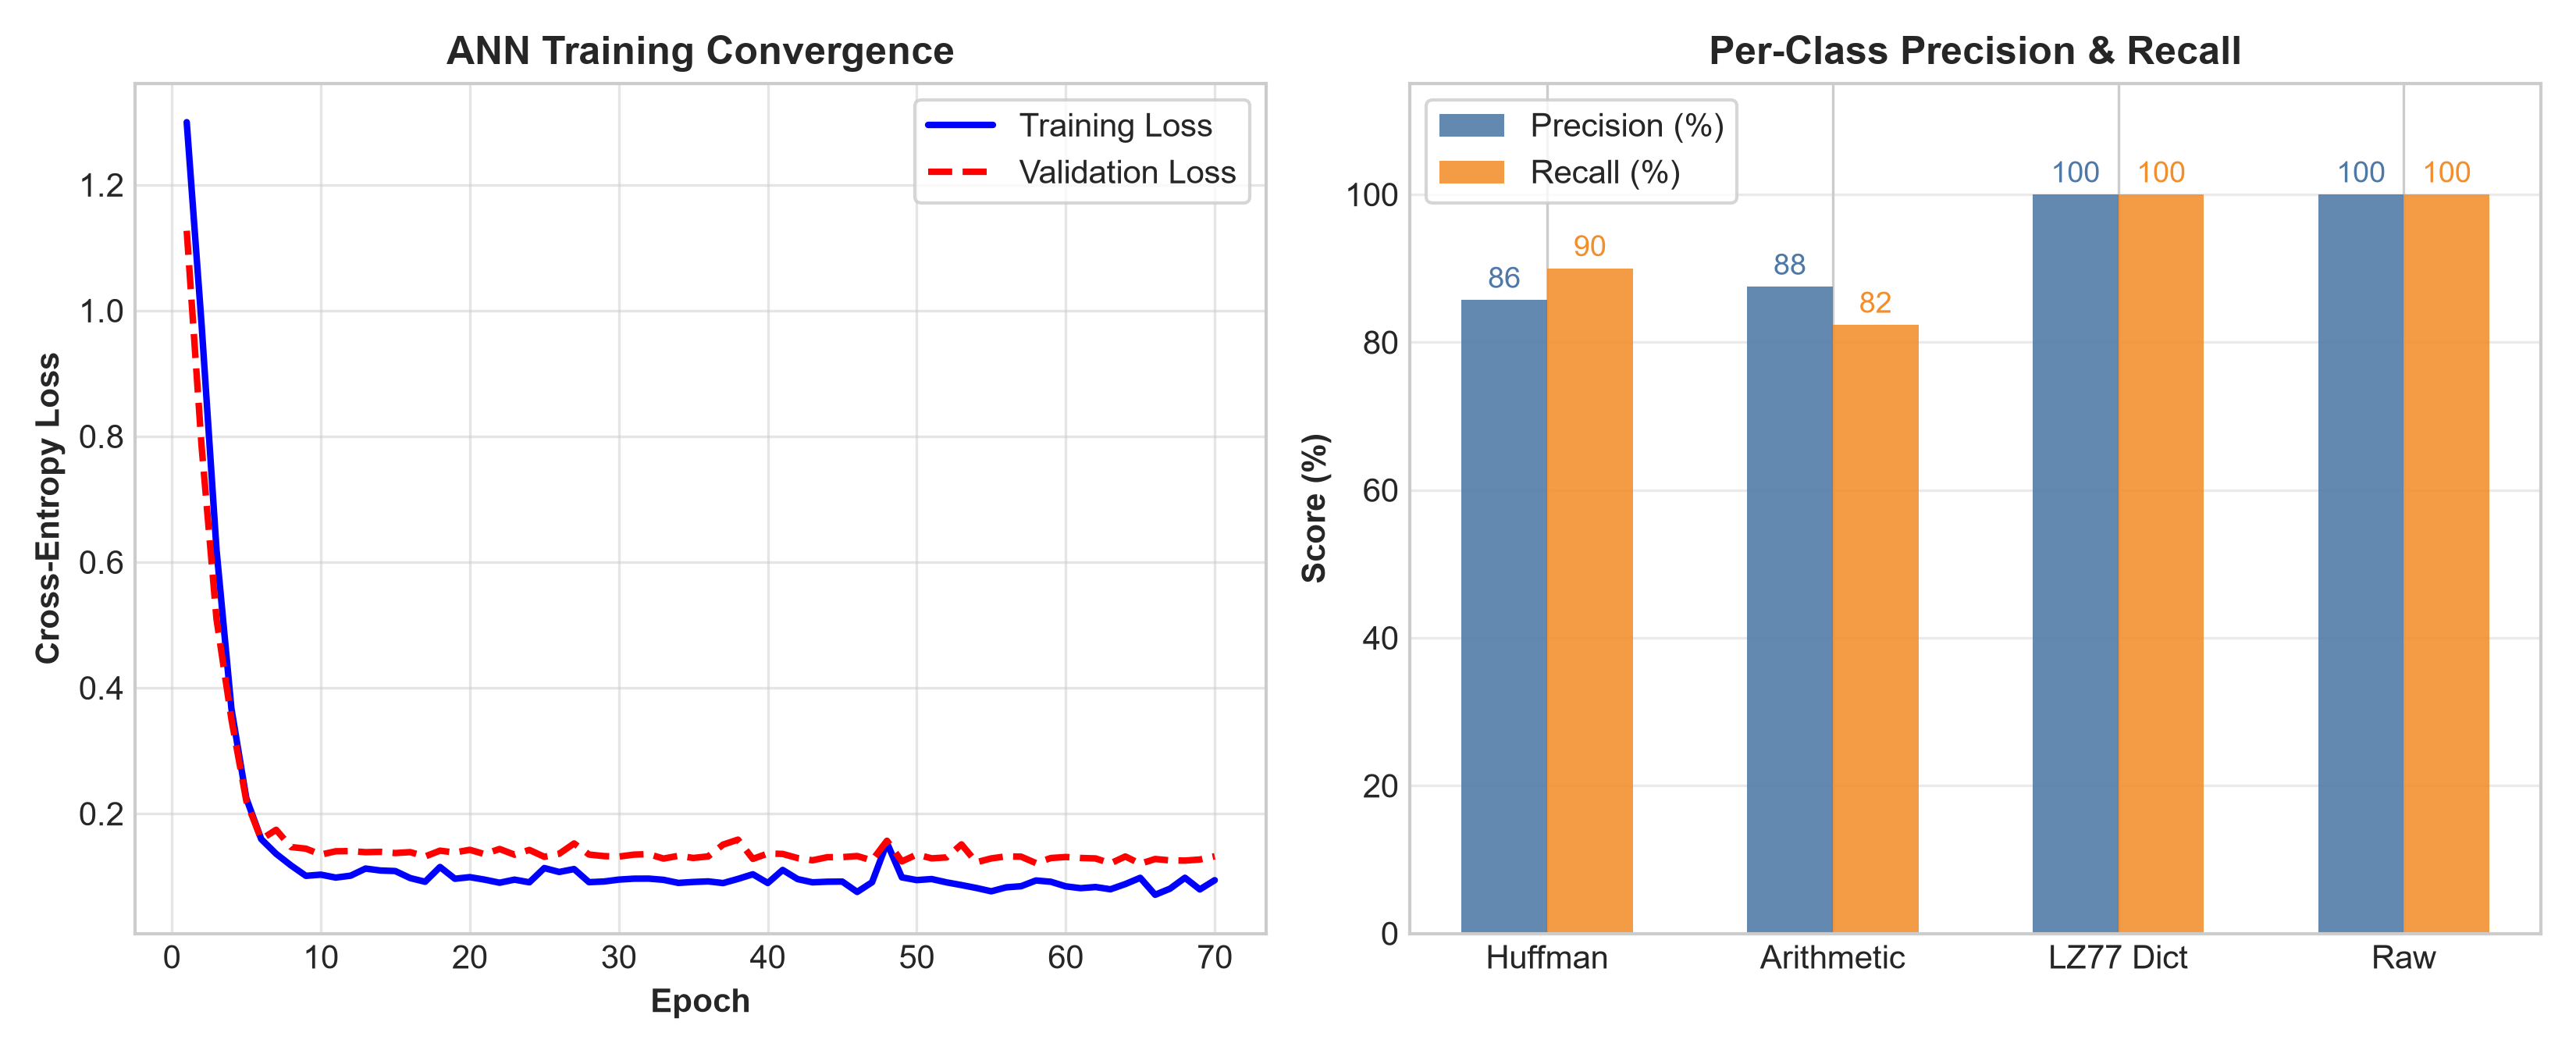
\includegraphics[width=\columnwidth]{results/fig4_learning_curves_and_class_metrics.png}
\caption{Left: ANN training and validation loss convergence over 70 epochs (AdamW with plateau LR scheduler). Right: per-class precision and recall on the held-out test set. LZ77 and Raw achieve perfect scores; Huffman/Arithmetic confusion is bounded by the 8-byte hysteresis threshold in the decision policy.}
\label{fig:learning_curves}
\end{figure}

\subsection{Scope and Methodological Limitations}
Five important limitations apply to the current evaluation:
\begin{enumerate}
    \item \textbf{Synthetic data bias}: The ANN's training labels derive from the same stochastic generation process as the test payloads. Deployed transceivers may encounter non-stationary traffic mixing multiple data types; future work should evaluate on empirical CAN-FD and PCIe traffic traces.
    \item \textbf{Short LDPC block length}: The $(128, 64)$ code has limited spatial diversity compared to moderate-length codes ($n \ge 1000$). Short-block LDPC codes exhibit higher error floors under mixed noise due to small trapping sets.
    \item \textbf{Variance normalization tight bound}: $\phi_2$ is normalized by $\sigma^2_{\max} = (255/2)^2 = 16256.25$ (the maximum variance of a binary $\{0, 255\}$ distribution), chosen to strictly bound $\phi_2 \in [0, 1]$.
    \item \textbf{Channel metric approximation}: The receiver employs a low-complexity Gaussian-mismatched LLR metric ($L(y_j) = 2y_j/\sigma^2$) rather than computing the transcendental Gaussian-Bernoulli mixture likelihood, trading asymptotic optimality under dense impulse noise for real-time hardware tractability.
    \item \textbf{Finite Monte-Carlo statistical resolution}: Evaluated within the $10^5$ coded channel bit simulation budget ($781$ blocks $\times 128 = 99{,}968$ coded bits), zero bit errors were detected across the $N_{\text{info}} = 49{,}984$ decoded information bits at $12.0\,\text{dB}$, establishing an empirical error rate of zero with a $95\%$ upper confidence bound of $6.0 \times 10^{-5}$. Validating BER levels below $10^{-7}$ requires hardware-accelerated FPGA emulation with $\ge 10^8$ channel bits.
\end{enumerate}

% =========================================================================
% SECTION V: CONCLUSION
% =========================================================================
\section{Conclusion}
\label{sec:conclusion}
This work presented an integrated joint source-channel coding framework for high-reliability wired communication. By combining an $O(N)$ statistical feature extractor with a lightweight MLP, the transmitter adaptively selects among Canonical Huffman, Integer Arithmetic, LZ77 Dictionary, and Raw Pass-Through coding in $\approx\!50\,\mu\text{s}$ per 2048-byte payload, attaining $93.33\%$ accuracy, $100\%$ Top-2 accuracy, and a mean compression regret of only $4.89$ bytes from the theoretical minimum. Across six diverse data domains, the adaptive engine achieves $2.55\times$ mean CR ($47.9\%$ bit savings), outperforming all static codecs while preventing bit inflation on incompressible data. Systematic $(128, 64)$ LDPC codes decoded via normalized Min-Sum BP achieve zero observed bit errors across $49{,}984$ decoded information bits at $12.0\,\text{dB}$ SNR (establishing a $95\%$ upper confidence bound of $\text{BER} \le 6.0 \times 10^{-5}$ via the Rule of Three) under combined AWGN and impulsive EMI. Future work will investigate hardware synthesis of the feature extractor on FPGA SerDes controllers, rate-compatible punctured LDPC codes for varying channel SNR, and online adaptive ANN retraining on live traffic statistics.

% =========================================================================
% REFERENCES
% =========================================================================
\begin{thebibliography}{00}

\bibitem{shannon1948}
C.~E. Shannon, ``A mathematical theory of communication,'' \textit{Bell System Technical Journal}, vol.~27, no.~3, pp.~379--423, Jul. 1948.

\bibitem{proakis2008}
J.~G. Proakis and M.~Salehi, \textit{Digital Communications}, 5th~ed. Boston, MA, USA: McGraw-Hill, 2008.

\bibitem{gallager1968}
R.~G. Gallager, \textit{Information Theory and Reliable Communication}. New York, NY, USA: John Wiley \& Sons, 1968.

\bibitem{mackay2003}
D.~J.~C. MacKay, \textit{Information Theory, Inference, and Learning Algorithms}. Cambridge, U.K.: Cambridge Univ. Press, 2003.

\bibitem{cover2006}
T.~M. Cover and J.~A. Thomas, \textit{Elements of Information Theory}, 2nd~ed. Hoboken, NJ, USA: Wiley-Interscience, 2006.

\bibitem{huffman1952}
D.~A. Huffman, ``A method for the construction of minimum-redundancy codes,'' \textit{Proceedings of the IRE}, vol.~40, no.~9, pp.~1098--1101, Sep. 1952.

\bibitem{rissanen1979}
J.~Rissanen and G.~G. Langdon, ``Arithmetic coding,'' \textit{IBM Journal of Research and Development}, vol.~23, no.~2, pp.~149--162, Mar. 1979.

\bibitem{witten1987}
I.~H. Witten, R.~M. Neal, and J.~G. Cleary, ``Arithmetic coding for data compression,'' \textit{Communications of the ACM}, vol.~30, no.~6, pp.~520--540, Jun. 1987.

\bibitem{ziv1977}
J.~Ziv and A.~Lempel, ``A universal algorithm for sequential data compression,'' \textit{IEEE Transactions on Information Theory}, vol.~23, no.~3, pp.~337--343, May 1977.

\bibitem{ziv1978}
J.~Ziv and A.~Lempel, ``Compression of individual sequences via variable-rate coding,'' \textit{IEEE Transactions on Information Theory}, vol.~24, no.~5, pp.~530--536, Sep. 1978.

\bibitem{welch1984}
T.~A. Welch, ``A technique for high-performance data compression,'' \textit{Computer}, vol.~17, no.~6, pp.~8--19, Jun. 1984.

\bibitem{deutsch1996}
P.~Deutsch, ``DEFLATE compressed data format specification version 1.3,'' RFC 1951, May 1996.

\bibitem{salomon2007}
D.~Salomon, \textit{Data Compression: The Complete Reference}, 4th~ed. London, U.K.: Springer-Verlag, 2007.

\bibitem{hamming1950}
R.~W. Hamming, ``Error detecting and error correcting codes,'' \textit{Bell System Technical Journal}, vol.~29, no.~2, pp.~147--160, Apr. 1950.

\bibitem{lin2004}
S.~Lin and D.~J. Costello, \textit{Error Control Coding}, 2nd~ed. Upper Saddle River, NJ, USA: Prentice-Hall, 2004.

\bibitem{gallager1962}
R.~Gallager, ``Low-density parity-check codes,'' \textit{IRE Transactions on Information Theory}, vol.~8, no.~1, pp.~21--28, Jan. 1962.

\bibitem{mackay1996}
D.~J.~C. MacKay and R.~M. Neal, ``Near Shannon limit performance of low density parity check codes,'' \textit{Electronics Letters}, vol.~32, no.~18, pp.~1645--1646, Aug. 1996.

\bibitem{richardson2001}
T.~J. Richardson and R.~L. Urbanke, ``The capacity of low-density parity-check codes under message-passing decoding,'' \textit{IEEE Transactions on Information Theory}, vol.~47, no.~2, pp.~599--618, Feb. 2001.

\bibitem{richardson2001design}
T.~J. Richardson, M.~A. Shokrollahi, and R.~L. Urbanke, ``Design of capacity-approaching irregular low-density parity-check codes,'' \textit{IEEE Transactions on Information Theory}, vol.~47, no.~2, pp.~619--637, Feb. 2001.

\bibitem{tanner1981}
R.~Tanner, ``A recursive approach to low complexity codes,'' \textit{IEEE Transactions on Information Theory}, vol.~27, no.~5, pp.~533--547, Sep. 1981.

\bibitem{fossorier1999}
M.~P.~C. Fossorier, M.~Mihaljevic, and H.~Imai, ``Reduced complexity iterative decoding of low-density parity check codes based on belief propagation,'' \textit{IEEE Transactions on Communications}, vol.~47, no.~5, pp.~673--680, May 1999.

\bibitem{chen2005}
J.~Chen, A.~Dholakia, E.~Eleftheriou, M.~P.~C. Fossorier, and X.~Hu, ``Reduced-complexity decoding of LDPC codes,'' \textit{IEEE Transactions on Communications}, vol.~53, no.~8, pp.~1288--1299, Aug. 2005.

\bibitem{zhang2010}
X.~Zhang and F.~Cai, ``Reduced-complexity min-sum algorithm for decoding LDPC codes,'' \textit{IEEE Transactions on Circuits and Systems I: Regular Papers}, vol.~57, no.~8, pp.~2099--2109, Aug. 2010.

\bibitem{o_shea2017}
T.~O'Shea and J.~Hoydis, ``An introduction to deep learning for the physical layer,'' \textit{IEEE Transactions on Cognitive Communications and Networking}, vol.~3, no.~4, pp.~563--575, Dec. 2017.

\bibitem{qin2019}
Z.~Qin, H.~Ye, G.~Y. Li, and B.-H. F. Juang, ``Deep learning in physical layer communications,'' \textit{IEEE Wireless Communications}, vol.~26, no.~2, pp.~93--99, Apr. 2019.

\bibitem{balle2018}
J.~Ball{\'e}, D.~Minnen, S.~Singh, S.~J. Hwang, and N.~Johnston, ``Variational image compression with a scale hyperprior,'' in \textit{Proc. Int. Conf. Learn. Represent. (ICLR)}, Vancouver, Canada, May 2018, pp.~1--14.

\bibitem{mentzer2019}
F.~Mentzer, E.~Agustsson, M.~Tschannen, R.~Timofte, and L.~Van~Gool, ``Practical full resolution learned lossless image compression,'' in \textit{Proc. IEEE/CVF Conf. Comput. Vis. Pattern Recognit. (CVPR)}, Long Beach, CA, USA, Jun. 2019, pp.~10629--10638.

\bibitem{sreekumar2020}
A.~Sreekumar, S.~Sreejith, and S.~R. V.~P, ``Machine learning for physical layer cognitive communications: A review,'' \textit{IEEE Communications Surveys \& Tutorials}, vol.~22, no.~4, pp.~2345--2372, 4th Quart., 2020.

\bibitem{alwarafy2022}
A.~Alwarafy, M.~Abdallah, B.~S. Ciftler, A.~Vukovic, and M.~Hefeida, ``Deep reinforcement learning for physical layer communications: Advances, challenges, and opportunities,'' \textit{IEEE Communications Surveys \& Tutorials}, vol.~24, no.~1, pp.~404--449, 1st Quart., 2022.

\bibitem{richardson2008}
T.~Richardson and R.~Urbanke, \textit{Modern Coding Theory}. Cambridge, U.K.: Cambridge Univ. Press, 2008.

\bibitem{3gpp38212}
\textit{Multiplexing and Channel Coding}, 3GPP Standard TS 38.212, V16.2.0, Jul. 2020.

\bibitem{lang2024}
A.~Lang and P.~Boncz, ``ALP: Adaptive lossless floating-point compression,'' in \textit{Proc. ACM SIGMOD Int. Conf. Management of Data}, Santiago, Chile, Jun. 2024, pp.~2274--2287.

\end{thebibliography}

\end{document}